\documentclass{report}

\usepackage[utf8x]{inputenc}
\usepackage[hidelinks]{hyperref}

\begin{document}
\pagenumbering{alph}
\title{256 Shades of gray}
\author{
Christer Emil Haga Bru\\
Vegard Edvardsen\\
Sondre Andreas Engebråten\\
Hans Kristian Flaatten\\
Martin Gammelsæter\\
Jean Niklas L'orange\\ % ' er før o i ASCII-tabellen
Erik Lothe\\
Andreas Steensnæs Morland\\
Mads Buvik Sandvei\\
Einar Johan Trøan Sømåen\\
Lichao Tang\\
Håkon Opsvik Wikene\\
Trygve Aaberge\\
}
\date{November 21, 2012}

\maketitle

\newpage
\thispagestyle{empty}
\mbox{}

\pdfbookmark[1]{Abstract}{Abstract}
\begingroup
\let\clearpage\relax
\let\cleardoublepage\relax
\let\cleardoublepage\relax

\chapter*{Abstract}
As heat generation and power consumption starts to limit speed and effectiveness
of single core architectures, parallelism is becoming more and more important
within all performance demanding computing. Everything from cell phones to
desktop computers now carries multiple processing cores to perform their
functions. Parallelism is of course not a new concept; for many decades,
exploiting the parallel nature of certain data to increate effectiveness in computation has
been a known strategy. Especially within the field of image processing,
parallelism has proved itself to be an extremely effective tool.

While \ac{MIMD} systems are dominant within general computing, we wanted to
explore alternatives which may work better for certain applications. The result
of this project is the computer ``256 Shades of Gray'', which is an array-based
\ac{SIMD} architecture optimized for massively parallelizable tasks such as
image processing.

256 Shades of Gray consists of a custom PCB design, a microprocessor operating
as a System Control Unit and an FPGA which implements our SIMD architecture. It
takes input through an SD card reader (with RS-232 and USB as backup), and shows
output through a custom VGA controller.

We have been inspired by the Goodyear MPP architecture, which clearly shows in
our design. Our main focus was performance, and because of that simplicity in
design has been strived for in order to fit as many parallel cores on our FPGA
as possible. As such, the SIMD nodes have been stripped of many
complex instructions, such as integer multiplication and division, as well as
all floating point capabilities. The SIMD array is controlled by a control core
that handles I/O and memory access through a DMA unit.

Our design has gone through testing and has met all functional and
non-functional requirements that were set. The architecture has shown itself
effective and well suited for common image processing tasks.
\endgroup



\chapter*{Acknowledgements}
\begin{itemize} % TODO: Fancy bulletpoints - or definition list
\item Magnus Jahre
\item Stefano Nichele
\item Gunnar Tufte
\item Lars-Ivar Hesselberg Simonsen % (???)
\end{itemize}


\pagenumbering{roman}
\tableofcontents
\listoffigures
\listoftables
\newpage
\pagenumbering{arabic}

\chapter{Introduction}\label{ch:intro}

\begin{flushright}{\slshape
    In which we introduce the reader to our project,\\
    our goal, our assumptions and how we will proceed,\\
    this being a good thing knowing before embarking
}
\end{flushright}

\section{Assignment}
The task given was to create an {\em array-based} parallel image processor with
focus on performance. An array processor is a grid of processing elements, where
each of the processing elements are only able to communicate with its north,
south, east, and west neighbors. All the processing elements will perform the
same instruction at all times, which means that the more processing elements one
has, the more data is processed simultaneously, leading to better performance.

Fast image processing is essential in robots\cite{miller1989r-vision,
  thrun2007stanley} and in artificial intelligence\cite{hwang1989parallel} in
order to work in the real world. Autonomous cars and robots need to process
images from image sensors fast enough to react and e.g. prevent
accidents\cite{aufrere2003coll-avoid}. Image processing in general is also
highly applicable in the medical field\cite{luong2009medical-image,
  sternberg1983biomedical} and in the petroleum
industry\cite{ferrari2007steam-images}.

\subsection{Original Assignment Text}

The original assignment was given as follows:

\begin{quotation}\em
The performance increase available from harvesting Instruction Level Parallelism
(ILP) from the serial instruction stream is limited because we have reached the
maximum power consumption that can be handled without expensive cooling
solutions \cite{olukotun2005future}. Consequently, there is a significant
interest in single-chip parallel processor solutions (e.g. \cite{bell2008tile64,
  kongetira2005niagara}).

The processor cores in commercial multi-core chips are conventional designs and
therefore reasonably complex. In this work, your task is to design an
array-based parallel image processor. An array processor is organized as a
matrix of processing elements where each element communicates with its neighbors
in the north, south, east and west directions.

Your image processor will be implemented on an FPGA, and you are free to choose
how to realize your array-based computer architecture. The system should be
shown to work with a suitable application. Studying the architecture of the
Goodyear MPP \cite{batcher1980design,wiki:goodyear} might be a possible starting
point.  Due to a large number of students this year, we will divide the work
into two independent projects: a) Performance and b) Energy efficiency. The goal
of group a) is to achieve maximum performance while group b) should try to
balance performance and energy. The reports from both groups should include an
evaluation of prototype performance and energy consumption.

\subsubsection*{Additional requirements}
The unit must utilize an Atmel AVR micro controller and a Xilinx
\acfoot{FPGA}. The budget is 10.000 NOK, which must cover components and
\acfoot{PCB} production. The unit design must adhere to the limits set by the
course staff at any given time. Deadlines are given in a separate time schedule.
\end{quotation}

\section{Requirements Specification}

\begin{table}[h]
  \centering
  \begin{tabularx}{\textwidth}{c X c}\toprule
    \thx{Name} & \thxc{Description} & \thx{Priority}\\ \midrule
    {\sc FR1} & \FRI   & {\sc High}   \\
    {\sc FR2} & \FRII  & {\sc High}   \\
    {\sc FR3} & \FRIII & {\sc High}   \\
    {\sc FR4} & \FRIV  & {\sc Medium} \\
    {\sc FR5} & \FRV   & {\sc Medium} \\
    {\sc FR6} & \FRVI  & {\sc Low}    \\
    {\sc FR7} & \FRVII & {\sc Low}    \\ 
    \bottomrule
  \end{tabularx}
  \caption[Functional requirements]{The functional requirements}
  \label{fig:func-req}
\end{table}

 A few functional
and most non-functional requirements were given to us by our instructor, Magnus
Jahre. The rest were decided by the group as goals we thought were realizable, and
some to help us see how far away we are from our goals. Table
\ref{fig:func-req}, which shows the functional requirements, includes a relative
priority between the different requirements.  This priority tells us what we
have focused on, as well as what is important in terms of success of the
computer. Clearly, focusing on performance, as specified in {\sc FR1}, is more
important than having developer tools for the machine ({\sc FR6}).

{\sc FR1} ensures a focus on performance. {\sc FR2} ensures that we do not end
up with a system that is not generally programmable. This is important, as a
machine hardcoded for certain image processing algorithms has less usability than a generally
programmable computer. {\sc FR3} and {\sc FR7} makes it easier to show that the
computer is capable of processing images, whereas {\sc FR4} through {\sc FR6} makes it
easier to use, debug and create programs for the computer.

\begin{table}[h]
  \centering
  \begin{tabularx}{\textwidth}{l X}\toprule
    \thxc{Name} & \thxc{Description}\\ \midrule
    {\sc NFR1} & The machine must use a Xilinx Spartan 3 XC3S500E PQG208 FPGA\\
    \midrule
    {\sc NFR2} & The machine must use one AVR32 UC3A microcontroller\\
    \midrule
    {\sc NFR3} & The budget of $\sim$ 10 000 NOK must cover all \ac{PCB} and
    component costs\\
    \midrule
    {\sc NFR4} & The image processor should consist of multiple cores arranged 
    in a matrix\\
    \midrule
    {\sc NFR5} & The machine should be optimized for performance\\
    \bottomrule
  \end{tabularx}
  \caption[Non-functional requirements]{The non-functional requirements}
  \label{fig:nonfunc-req}
\end{table}


Table \ref{fig:nonfunc-req} shows the non-functional requirements. These were
all determined by the assignment. They were all treated as absolute requirements,
and our design has been centered around these. {\sc NFR1} and {\sc NFR2} gave us
little choice in what hardware to use, and naturally this hardware has been used. {\sc
  NFR3} limits us to use inexpensive components. {\sc NFR4} constrains our
design choices when designing the image processor. We could not make any type of core
organization, we had to make this specific type. {\sc NFR5} leads to some
design choices for the entire system. Our goal was to get the best possible performance, and we did not
have to care about concerns such as energy consumption. 
However, we may have sacrificed some simplicity in our design for
the sake of performance.

\section{Terminology, Names and Conventions}
The following acronyms are used consistently throughout the report, to ease
reading: \CHECK{Should this be in background?}

\begin{description}
\item[PCB] Printed Circuit Board
\item[AVR] Not an acronym, but a microprocessor architecture
\item[FPGA] Field-Programmable Gate Array
\item[SIMD] Single Instruction, Multiple Data \TODO{Make abbr. tt instead?}
\item[RISC] Reduced Instruction Set Computer
\item[VGA] Video Graphics Array
\item[ALU] Arithmetic Logic Unit
\item[USB] Universal Serial Bus
\item[I/O] Input/Output
\item[JTAG] Joint Test Action Group
\item[API] Application Programming Interface
\item[RAM] Random Access Memory
\item[SRAM] Static Random Access Memory
\item[DRAM] Dynamic Random Access Memory
\item[SD] Secure Digital
\end{description}

\section{Structure of the Report}

This report may be seen as split up in three different parts: chapters
\ref{ch:intro}, \ref{ch:sys-over}-\ref{ch:pcb} and
\ref{ch:sys-test}-\ref{ch:conc}. The
current chapter has given you an introduction to the assignment and our goals.
% and our team. \CHECK{Is the background chapter included?}
% Chapter \ref{ch:back} contains relevant background information for
% reading the rest of the report.

Chapters \ref{ch:sys-over} to \ref{ch:pcb} explains in deeper detail {\em how}
the machine works. Chapter \ref{ch:sys-over} gives an overview of the whole
machine and how the different parts are connected together. Chapter
\ref{ch:fpga} elaborates on the \ac{LENA} Architecture, which is the \ac{FPGA}
design of the machine. \ac{SIMD} nodes, control core as well as the \ac{FPGA}
\ac{VGA} module is explained in detail, along with the interconnection between
these. Chapter \ref{ch:avr} describes the software and structures for the AVR,
such as the file format and the program and data menu. Chapter \ref{ch:pcb}
explains the work with designing the \ac{PCB}, as well as the soldering and
other workarounds we had to do.

Chapters \ref{ch:sys-test} to \ref{ch:conc} is the conclusion part of the
report. Here we test the machine, discuss our choices and present our
conclusion, as well as possible further work. Chapter \ref{ch:sys-test} contains
tests to check whether we have managed to reach our requirements or not, along
with their results. Chapter \ref{ch:res} describes the result, performance and
energy consumption of the machine with different cores and different
programs. Chapter \ref{ch:disc} discusses different choices we did in our
project, and the result of these. In chapter \ref{ch:conc}, our conclusion is
given along with further work.


% Background (?)
\chapter{System Overview}\label{ch:sys-over}

\begin{flushright}{\slshape
    In which a complete overview of the system is given,\\
    giving us a better understanding of how\\
    all the components are connected
}
\end{flushright}

\section{System Architecture}

A general concern when designing large systems is the accidental
complexity\cite[p.~8-9]{holt2004uml} one may create by poor design choices early
on. Many solutions designed to reduce accidental complexity are based around
software systems, and sacrifices performance in both the time domain and in the
space domain\cite{moseley2006out}. While these solutions may be applicable
within hardware systems where these kinds of performance degradations are not a
problem, it is unacceptable in systems where one or multiple of the system
requirements are a performance increase in one or both of these domains. As one
of our main requirements is focus on performance, we have to accept a certain
level of inherent complexity.
\begin{figure}[h]
  \centering
  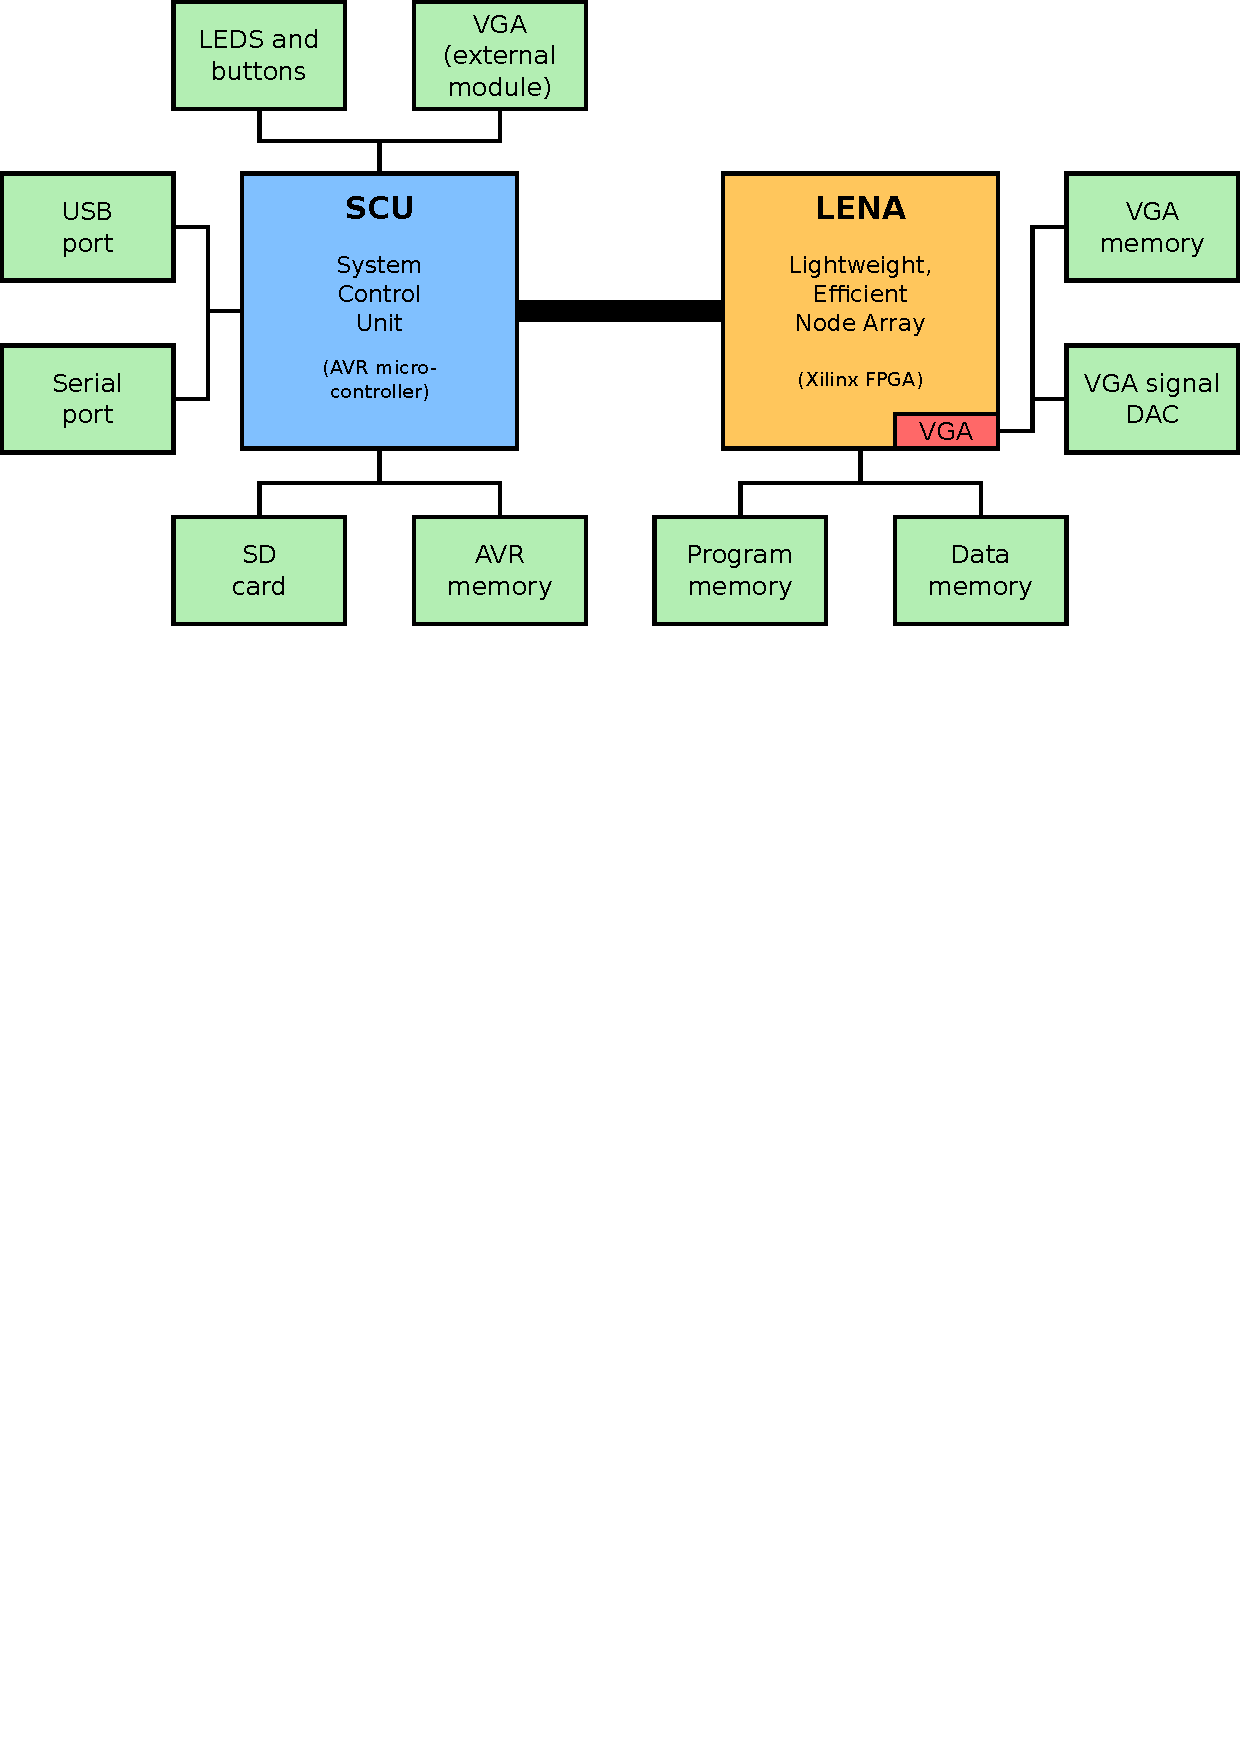
\includegraphics[width=\linewidth,clip,trim=0 18cm 0 0]
                  {fig/sys-over/arch-fig.pdf}
  \caption{System Architecture}
  \label{fig:sys-over-arch-fig}
\end{figure}


To remedy the complexity which inevitably follows from our requirements, we
focused on making it possible to isolate errors and make it possible to test
the individual components as early as possible: The \ac{LENA} architecture was
tested through \ac{VHDL} test benches, the \ac{VGA} component was tested with
prototypes on a breadboard, and the \ac{SCU} was tested with an EVK1100 development
board as well as with the buttons and \ac{LED}s on the PCB once it arrived.
By doing this, we could assume that errors occurring when connecting different
components are mostly due to errors in the protocol implementation(s).

Figure \ref{fig:sys-over-arch-fig} shows our resulting architecture. We also included a
\ac{VGA} connector connected to the AVR, in case the \ac{LENA} architecture
should fail to implement its \ac{VGA} module.

To be able to process data, we needed an \ac{I/O} device which could serve the machine
with data it should process. To ensure that we would have at least one
functional \ac{I/O} component,\CHECK{Sounds okay now?} we included both a serial
port, a \ac{USB} port and an \ac{SD} card reader on the \ac{PCB}. In addition,
to be able to keep enough data in memory and allow full overlap of different memory
transactions to make processing fast, the \ac{LENA} architecture has three separate
memory components. One for \ac{VGA}, one for instructions and one for data.

\section{Component Functionality}

This section describes the different components and their functionality. A list
of ordered parts can be found in \ref{app:ordered-parts}.
\TODO{Jahre vil ha figur(er)}

\subsection{System Control Unit}

The \acf{SCU} is used to control the \ac{LENA} architecture and as a user interface.
The SCU sends data and instructions from the \ac{SD} card to \ac{LENA}, which stores
it in it's data and instruction memory respectively. The \ac{SCU} also starts and stops \ac{LENA}'s program.

Selecting programs and data is done by the user interface on the \ac{SCU} using buttons as input
and \ac{LENA}'s VGA as output. 

\subsection{LENA}

NF4 constrained our high level choices on the image processor architecture:
There was a requirement that we had to have multiple cores arranged in a
matrix. As the matrix would perform image processing, it was natural for us to
choose a \ac{SIMD} architecture. Many image processing algorithms do the exact
same operation on every pixel, and having a \ac{SIMD} architecture reduces both
complexity and size needed per core on the \ac{FPGA} significantly.

Other design choices that followed was the introduction of a control core, a
\ac{DMA} and a \ac{VGA} controller. The control core is responsible for sending
data to the \ac{SIMD} nodes and the \ac{VGA} controller, whereas the \ac{DMA} is
responsible for writing data from the \ac{SIMD} nodes back into memory. The
\ac{VGA} controller is responsible for handling the \ac{VGA} memory and sending
the correct signals to the \ac{VGA} port. In addition, as the \ac{SIMD} nodes
usually depend heavily on their neighbor's data, we decided to have ``dummy
nodes'' outside the real \ac{SIMD} nodes. Their only function is to transmit
data to the edge nodes. As such, we can still utilize the edge nodes for
computation when neighbor data is needed.

\subsubsection{Memory}
The memory is split over three different chips: The data memory, the
instruction memory and the \ac{VGA} memory. All of the \ac{RAM} is asynchronous
\ac{SRAM}, based on previous projects success with
it\cite{berg2011festinalente} along with the speed. The main reason for this
choice was mostly due to frequent reading and writing, but also because a
larger \ac{SRAM} module was more costly than multiple smaller \ac{SRAM} modules
per \ac{MB}. An additional benefit from this is that the complexity is lowered:
Fewer potential collisions on \ac{RAM} reading and writing occurs since fewer
parts read and write to the different \ac{RAM} chips.

\subsubsection*{Instruction Memory}
We ended up with a 24-bit instruction set for both \ac{SIMD} nodes and the
control core. As we ended up with a 16-bit program counter, the maximal
instruction count would be 64,000 and the memory chip size is chosen on that
basis. While it may sound little, it is still more than enough. To see why,
note that the control core can start the image processing algorithm from the
beginning when the \ac{SIMD} nodes have finished processing the current data.
Also, we usually define algorithms for a single frame, without any concern
for the one coming after it. The program is simply restarted for every new frame,
reducing the amount of code needed and the complexity of the programs.

\TODO{Isn't both data- and vga memory discussed in length later in the report?}
\subsubsection*{Data Memory}

\subsubsection*{VGA Memory}

\subsection{I/O}




\chapter{The LENA Architecture}\label{ch:fpga}

\begin{flushright}{\slshape
    In which hardware is reconfigured and set up\\
    to perform a single instruction multiple times\\
    each time with different data, simultaneously
}
\end{flushright}

\section{SIMD nodes}

\ac{SIMD} nodes are the main processing cores of the image processor and are
responsible for carrying out data processing-instructions in paralell. They
share the same instruction set and executes the same instruction, hence
\acf{SIMD} and operates on an 8-bit word size, as most of the processor does.

Each \ac{SIMD} node is fully equipped with a register bank, an \ac{ALU}, message
passing with adjacent nodes and an instruction decoder for the \ac{SIMD} node
instruction set, explained in detail in subsequent section.

The schematic of a single \ac{SIMD} node is shown in figure
\ref{fig:fpga-simd-arch} details the entire datapath for the node. Different
parts of the instruction and other inputs and outputs to and from the node are
all labled with red lables. In this section we will reffer to this image when
explaining the different components.

\TODO{Fix signal labels in arhitecture image to differentiate between input, output and instruction}

\begin{figure}[h]
  \centering
 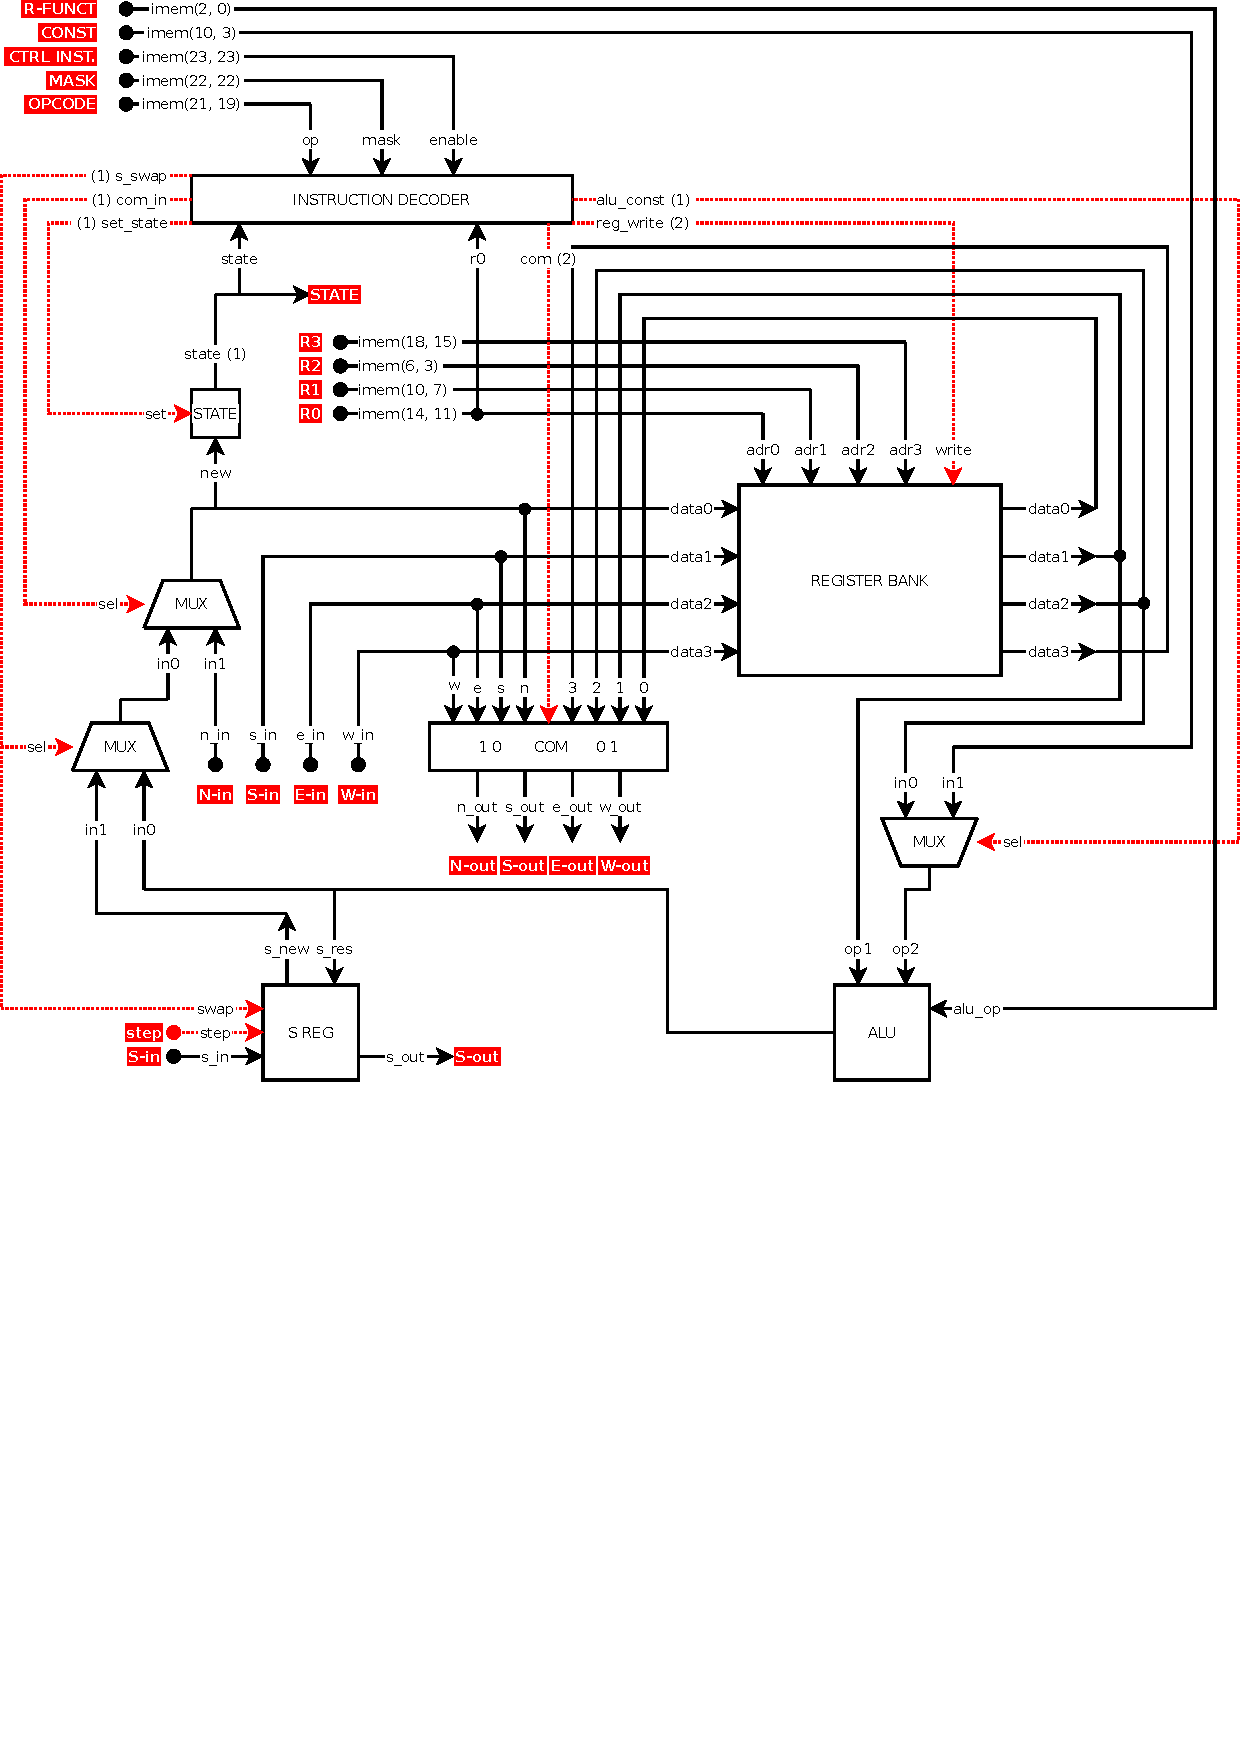
\includegraphics[width=\linewidth,clip,trim=0 0 0 0]
                  {fig/fpga/fpga-simd-arch.pdf}
  \caption{LENA SIMD architecture}
  \label{fig:fpga-simd-arch}
\end{figure}


\subsection{Components}

\TODO{This pharagraph is kind of VHDL implementation specific. Should we keep it?}

In order to the keep the ammount of intermediate signals to a minimum, as well
as better reusability accross other parts of the processor, the \ac{SIMD} node
is nicely divided into separate, stand-alone, components which when linked
together makes up the datapath for the node.

\subsubsection{Instruction Decoder}

\TODO{List all the different OP-codes and their meaning.}

When an instructions is first recieved by a \ac{SIMD} node the first 5-bits
(enable, mask and opcode) are fed directly into the Instruction Decoder. The
decoder will then set up the correct control signals other components based on
the current state of the \ac{SIMD} node and instruction opcode.

\subsubsection{Communication}
The Communication component controlls outbound data from the \ac{SIMD} node to
adjacent \ac{SIMD} nodes in the grid array. It can either send data from 4
registers out on north-, south-, east- and west-bound links, forward incoming
links in an clockwise spiral according to \ref{fig:fpga-simd-datacom} or keep
the previously outgoing data. The latter is very important in order for
branching to work correctly; where some \ac{SIMD} nodes, depending on their
state, may store incoming data in one register and others \ac{SIMD} nodes in an
other register.

The clockwise spiral forwarding is an optimized way of distributing a 3x3 array
of source data to all the \ac{SIMD} nodes in the grid array using only 3-clock
cycles. \TODO{We made this one ourselves! note that down}

\subsubsection{Register Bank}
Each \ac{SIMD} node is equpped with $2^4 = 16$ general purpose registers. 14 of
which are available for general storage during acecution. The remaining 2 are
reserved for the special purpose registers {\tt \$zero} and {\tt \$state}.

\begin{table}[h]
  \centering
  \begin{tabularx}{\linewidth}{XXXXXXXXX}\toprule
    R0 & R1 & R2 & R3 & R4 & R5 & R6 & R7 \\ \midrule
    \tt \$zero & \tt \$r1 & \tt \$r2 & \tt \$r3 & \tt \$r4 & \tt \$r5 &
    \tt \$r6 & \tt \$r7\\ \bottomrule
  \end{tabularx}
  \begin{tabularx}{\linewidth}{XXXXXXXX}
    R8 & R9 & R10 & R11 & R12 & R13 & R14 & R15 \\ \midrule
    \tt \$r8 & \tt \$r9 & \tt \$r10 & \tt \$r11 & \tt \$r12 & \tt \$r13 &
    \tt \$r14 & \tt \$state\\ \bottomrule
  \end{tabularx}
  \caption{Registers in the SIMD nodes}
  \label{tab:simd-registers}
\end{table}


The register bank has specially designed with the four way data transfer in
mind. It supports reading, or writing, 4 registers at once or reading 2
registers and writing 1 register within one clockcycle.

\subsubsection{Arithmetic Logic Unit}

\TODO{List the 8 ALU functions some where with their binary prepresentation.}

The \ac{ALU} implemented is a very simple {\tt 8}-bit \ac{ALU} supporting only 8
instructions. The main reason for only implementing the most basic arithmetic
instruction was to save space in the instruction set, since all \ac{SIMD} node
instructions carries the 3-bit \ac{ALU} function at the end, and to reduce the
pysical size of the node.

\TODO{Add some supporting references.}

Upon investigating image processing algorithmes we found that many of these,
Median Filter and Salt and Pepper noice reduction, only need these 8 \ac{ALU}
operations in order to perform their work. Besides; more high level arithmetic,
such as multiply and divide, can be implemented using addition and subtraction.

\subsubsection{Source Data Register}
The source data register (S REG), is a special purpose register within the
\ac{SIMD} node which holds the next source data for the \ac{SIMD} node. It is
partly controlled by the \ac{SIMD} node instruction set and partly by a special
{\tt step} signal sent from the \ac{DMA}.

An important attribute of the S REG is its capability to receive data from the
left node and passing it along to node on the right when instructed by the {\tt
  step} signal. This allows for a simultaneous data transfer while the node is
otherwise busy processing.

\subsubsection{State Register}
In order to handle branches the \ac{SIMD} node must have some internal
state. The State Register is, as all other registers, 8-bit. The least
significant bit is the current state wich is sent out from the node and to the
Instruction Decoder unit within the \ac{SIMD} node.

The State Register can be written and read as any other register in the Register
Bank and the state can hence be shifted left or right in order to acheave nested
branches.

\subsection{BRAM and SRAM}

\TODO{Where to put this?}

\ac{BRAM} or \ac{SRAM} is not available from the \ac{SIMD} node.

\subsection{Instruction Set}

\begin{figure}[h]
  \centering
  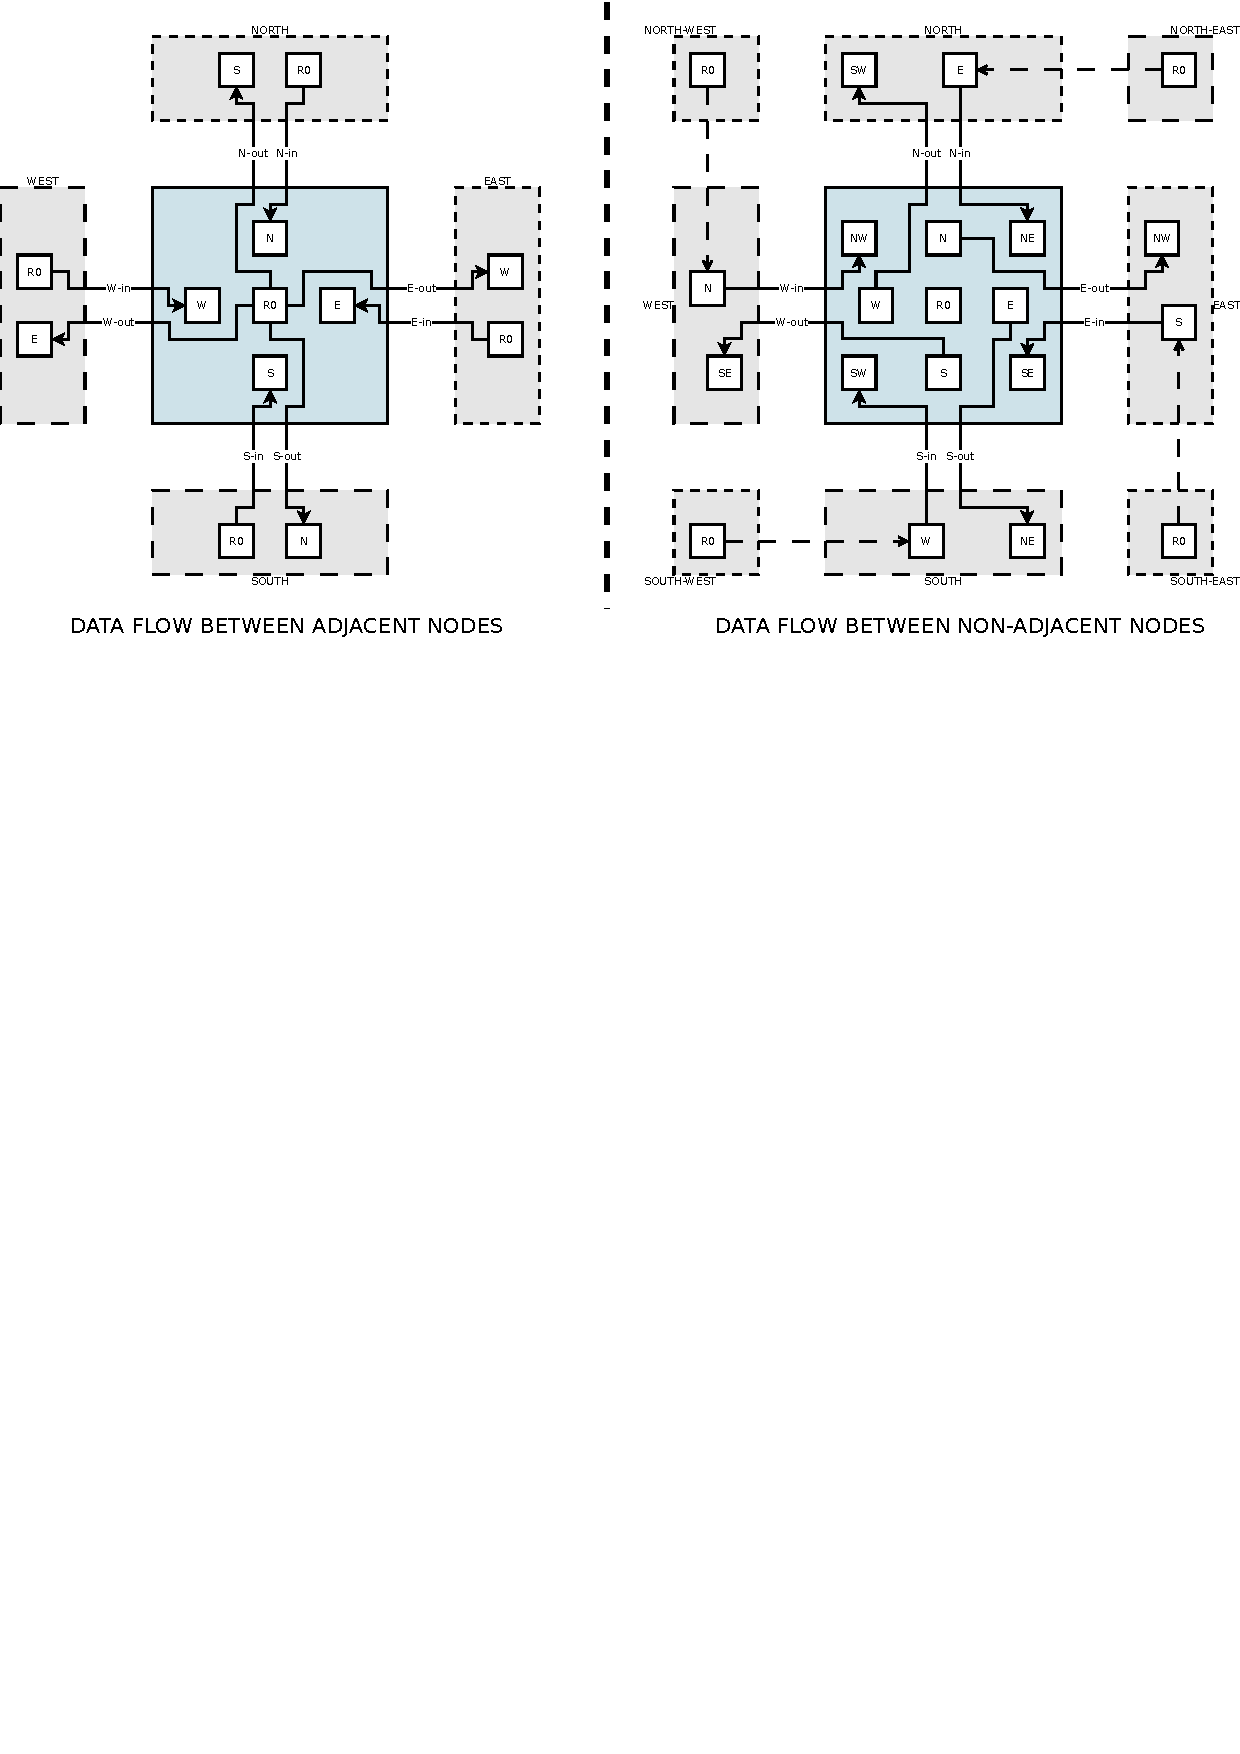
\includegraphics[width=\linewidth,clip,trim=0 18cm 0 0]
                  {fig/fpga/fpga-simd-datacom.pdf}
  \caption{Four-way communication in the LENA SIMD array.}
  \label{fig:fpga-simd-datacom}
\end{figure}


\subsection{Branching}
\CHECK{Should this be added to the appendix or something?}

Since all nodes run the same instructions, both parts of a branch must be
executed. Nodes are setting the {\tt state} to 1 in order to indicate that they
are executing within that part of the branch.

\begin{table}[h]
  \centering
  \begin{tabularx}{\textwidth}{rlcX}\toprule
    \thxc{step} & \thxc{instruction} & \thxc{state} & \thxc{description} \\
    \midrule
    0 & \tt // initial state & 0 & \\
    1 & \tt eq \$state \$r1, \$r2 & 1
    & Set state to 1 if branch should be taken for the node.\\
    \ldots & \tt // branch taken & 1 &
    Instructions for when the branch is taken.\\
    2 & \tt eq \$state, \$state, \$zero & 0 & Negate the state.\\
    \ldots & \tt // branch not taken & 0 & Instructions for when the branch is
    not taken.\\ \bottomrule
  \end{tabularx}
  \caption{Single level branching}
  \label{tab:single-level-branching}
\end{table}


\subsubsection{Multilevel branching}
Since state register is 8 it is possible to have up-to 8 nested branches by
shifting the current state to the left and adding the new state to the
end. Below \TODO{Refer to table, not relative to where it is placed} are the
instructions for performing a multilevel-branch.

\CHECK{Better switch out zeroes and ones with x'es and y's?}
\begin{table}[h] % TODO: Drag out
  \centering
  \begin{tabularx}{\textwidth}{rlcX}\toprule
    \thxc{step} & \thxc{instruction} & \thxc{state} & \thxc{description} \\
    \midrule
    0 & \tt // initial state & 01 & \\
    1 & \tt sll \$r3, \$state & 01
    & Save the current state by shifting left.\\
    2 & \tt eq \$r4 \$r1, \$r2 & 01
    & Calculate if branch is taken for the node.\\
    3 & \tt add \$state \$r4, \$r3 & 11
    & Set the new state.\\
    \ldots & \tt // branch taken & 11 &
    Instructions for when the branch is taken.\\
    4 & \tt andi \$r3, \$state, 1111 1110 & 11
    & Save the old state for the node.\\
    5 & \tt andi \$r4, \$state, 0000 0001 & 11 & Save the current state.\\
    6 & \tt eq \$r4, \$r4, \$zero & 11 & Negate the current state.\\
    7 & \tt add \$state, \$r4, \$r3 & 10 & Set new state.\\
    \ldots & \tt // branch not taken & 10
    & Instructions for when the branch is not taken.\\
    8 & \tt srl \$state, \$state & 01 & Revert to state before branch by
    shifting right.\\ \bottomrule
  \end{tabularx}
  \caption{Multi level branching}
  \label{tab:multi-level-branching}
\end{table}

\CHECK{Could any of these tables be figures instead?}

\section{VGA controller}

We learned early on that last years' group had problems with their off-the-shelf
\ac{VGA} controller being a major bottleneck, and were only able to squeeze out
less than one frame per second. Since one of our goals (FR1, Table
\ref{fig:func-req}) with this project was to hit a minimum frame rate of ten
frames per second, using a similar approach would most likely leave us with a
machine unable to fulfill FR1.

After having scoured the Internet for higher performing \ac{VGA} controllers in our
price range without any luck, and after consulting with Jahre, we decided to
implement our own \ac{VGA} controller on the \ac{FPGA}.

\section{VGA controller}

We learned early on that last years' group had problems with their off-the-shelf
\ac{VGA} controller being a major bottleneck, and were only able to squeeze out
less than one frame per second. Since one of our goals (FR1, Table
\ref{fig:func-req}) with this project was to hit a minimum frame rate of ten
frames per second, using a similar approach would most likely leave us with a
machine unable to fulfill FR1.

After having scoured the Internet for higher performing \ac{VGA} controllers in our
price range without any luck, and after consulting with Jahre, we decided to
implement our own \ac{VGA} controller on the \ac{FPGA}.

\input{fig/fpga/vga}

\subsection{Design}
We recognized the importance of allowing the control core to dump pixels to the
\ac{VGA} controller at its own pace without having to meet certain timing criteria,
so a physical memory and hence a memory controller was needed. Since the \ac{FPGA}
is running on 50MHz \TODO {This is wrong, system runs on 25MHz} and the pixel clock should be running on approximately
25MHz, a fairly simple solution for dividing the memory between the control
core and the actual signal generator was found: The signal generator must be
able to read from memory at most every other cycle, so the remaining cycles are
all free for the control core to use. To simplify the design as much as
possible, the memory controller simply alternates every cycle between writing
what is asserted on the signals from the control core, and reading a pixel
for the signal generator.

The signal generator itself is pretty straightforward. It calculates
when to pulse the V-sync and H-sync signals for a given resolution, and outputs
a (8-bit greyscale) pixel fetched from the memory controller at the appropriate
time.

\subsection{Circuitry}
\input{fig/fpga/vga-circuit} 

When designing the circuit, we had to choose between a black box \ac{DAC} and
making our own. Preliminary research on the \ac{VGA}-protocol showed that for
our purposes and our fairly low requirements on quality, making the \ac{DAC}
with simple resistors in parallel would be sufficient. Each resistor doubles in
resistance for each step from the most significant bit to the least
significant. We thought this would be easier to prototype and debug. The
resulting circuit is shown in Figure \ref{fig:vga-circuit}. Since color was a
``nice-to-have'' in case we had time to spare and not at all a priority, we made
the decision to greatly simplify the design by making the switch from greyscale
to color a manual operation of moving a set of jumpers. This way we reduced both
pin usage on the \ac{FPGA} and the complexity of the circuit.


\subsection{Design}
We recognized the importance of allowing the control core to dump pixels to the
\ac{VGA} controller at its own pace without having to meet certain timing criteria,
so a physical memory and hence a memory controller was needed. Since the \ac{FPGA}
is running on 50MHz \TODO {This is wrong, system runs on 25MHz} and the pixel clock should be running on approximately
25MHz, a fairly simple solution for dividing the memory between the control
core and the actual signal generator was found: The signal generator must be
able to read from memory at most every other cycle, so the remaining cycles are
all free for the control core to use. To simplify the design as much as
possible, the memory controller simply alternates every cycle between writing
what is asserted on the signals from the control core, and reading a pixel
for the signal generator.

The signal generator itself is pretty straightforward. It calculates
when to pulse the V-sync and H-sync signals for a given resolution, and outputs
a (8-bit greyscale) pixel fetched from the memory controller at the appropriate
time.

\subsection{Circuitry}
\begin{figure}[h!]
\centering
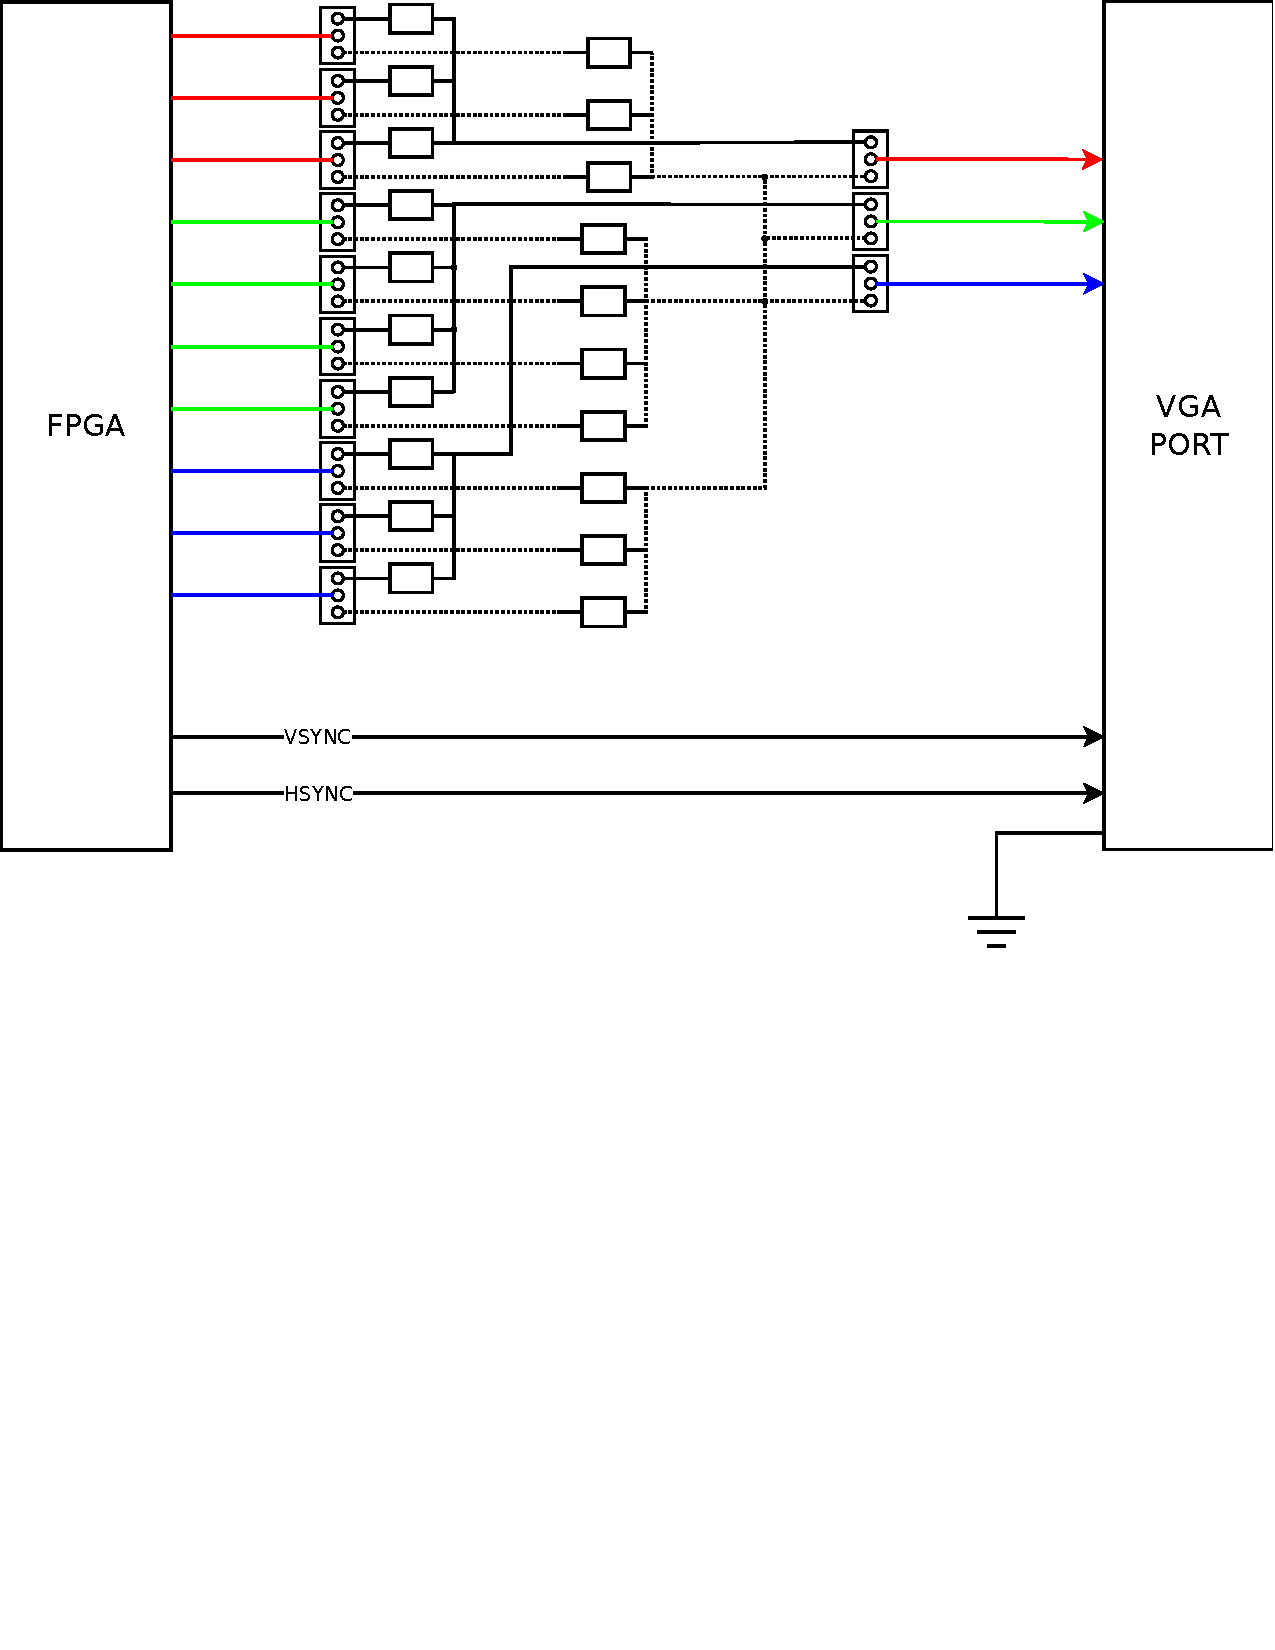
\includegraphics[width=\linewidth,clip,trim=0 11cm 0 0]
                {fig/fpga/vga-circuit.pdf}
\caption[VGA controller]
        {The resistor network of the DAC.}
\label{fig:vga-circuit}
\end{figure}
 

When designing the circuit, we had to choose between a black box \ac{DAC} and
making our own. Preliminary research on the \ac{VGA}-protocol showed that for
our purposes and our fairly low requirements on quality, making the \ac{DAC}
with simple resistors in parallel would be sufficient. Each resistor doubles in
resistance for each step from the most significant bit to the least
significant. We thought this would be easier to prototype and debug. The
resulting circuit is shown in Figure \ref{fig:vga-circuit}. Since color was a
``nice-to-have'' in case we had time to spare and not at all a priority, we made
the decision to greatly simplify the design by making the switch from greyscale
to color a manual operation of moving a set of jumpers. This way we reduced both
pin usage on the \ac{FPGA} and the complexity of the circuit.


\chapter{AVR}


\chapter{PCB}\label{ch:pcb}

\begin{flushright}{\slshape
    Electricity is really just organized lightning.\\ \medskip
    --- George Carlin}
\end{flushright}

\begin{figure}[h]
  \centering
  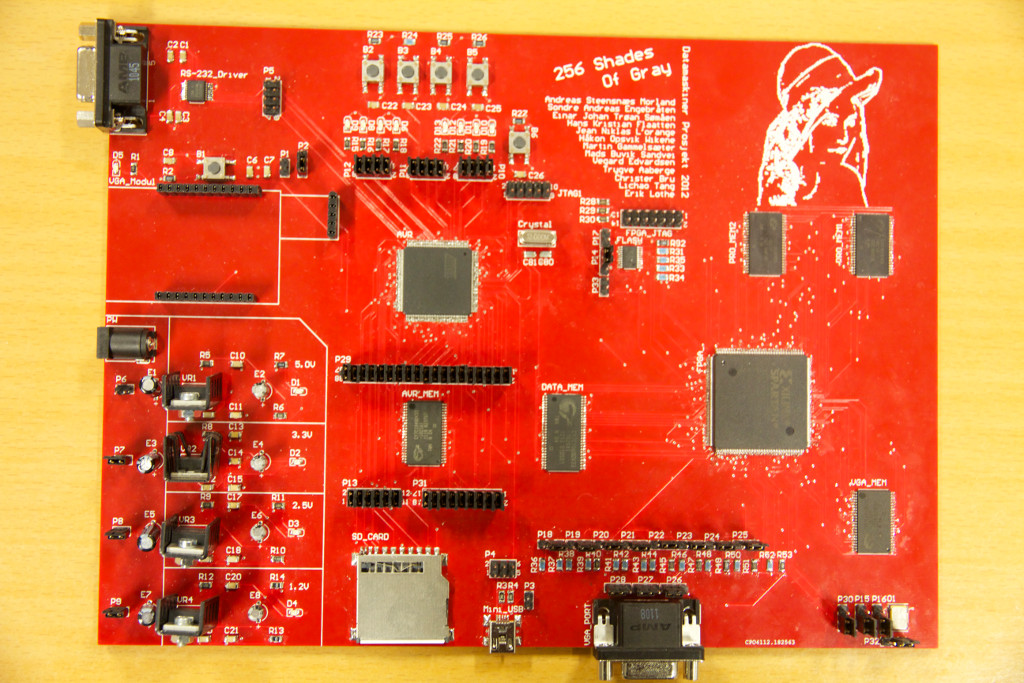
\includegraphics[width=0.8\textwidth]{fig/pcb/pcbwithcompnew.jpeg}
  \caption[The PCB]{The PCB With All The Components.}
  \label{fig:pcb-with-components}
\end{figure}

The entire system is connected together on the PCB. Designing and soldering
a correct and working PCB is thus important to be able to construct the system
as a whole.

This chapter will start by explaining how some of our overall design choices
affected the PCB design. We elaborate our power layout before giving an
overview of where we got our footprints from. We then go through how the PCB was
tested. Finally, we explain the process of making the PCB, as well as some of
the issues and solutions we met during the process.


\section {Introduction}

Design choices: \\
\subsection {Memory}
Since we decided to have separate instruction/data-memories, as well as VGA-ram, and
a dedicated memory for the AVR, we ended up with a total of 5 RAM-chips. The requirements
on the various chips did differ a bit though, we needed 8-bit words for all data, but
24 bit for instructions. Since 24-bit memory was out of production, and 32-bit memory
was too expensive, we opted for using two 16-bit chips, with their address-lines connected
together, and 8 ignored I/O-pins, thus in effect creating a 24-bit memory. Additionally,
as we were unsure about how constant we could get our data-streams, an additional
AVR-memory was added. This was chosen to be the same chip as the VGA-memory.

\subsection {VGA}
While we had a goal of creating our own VGA-controller in the FPGA, we decided to have
some fallback-option, thus, in addition to the neccessary pins and connectors for that
solution, we also added the necessary connectors for the VGA-module that Festina Lente
used last year.

\subsection {Communication}
We planned on using the SD-Card-reader as our main source of data/instructions, however
in the same vein as the design choices for the VGA, we opted to also have a fallback-solution
here, thus we also added USB and RS232 as fallback-solutions for getting data/communicating
with the computer.


%Flytta til process
%\subsection {Schematics}
The workflow of creating the schematic consisted of reading data sheets,
and looking at the reports from earlier computer design projects, and then
applying the knowledge we found from those to properly place the necessary
components in our schematic.

We decided to design the entire \ac{PCB} in one schematic, as the Festina Lente
report mentioned that Festina Lente-report does mention that 
``The decision to make the central components appear in multiple schematic
sheets made Altium issue a lot of warnings and errors during the design rule 
check''\cite[p.~49]{berg2011festinalente}. Something we avoided from day one, 
as we never attempted to use multiple schematics-documents.

A downside of this approach was the fact that this partially serialized
our work on the schematic, since we could not make concurrent changes to our
single document. When not working on the schematic, the other people in the
\ac{PCB} group did whatever could be done without touching the
schematic. (Making footprints, verifying design, looking up parts and data
sheets) Since the schematic was the biggest amount of work, this produced
something of a bottleneck for the PCB work.

However, having overall control of the entire thing in one document
did help to smooth out some issues we met while working. For instance,
we were having quite a few issues with net labels. This was quite easy to
solve when everything was in one document with no ports, as getting
complete overview was doable, without having to cross-reference schematics.
We also avoided the need to use any buses, although we did end up adding
some for the sake of readability.

The overall layout of the Schematic \ref{app:schematics} is logically grouped ``geographically'', to
allow for easy reading of the schematic.

\subsubsection {Buses/Wirelabels}
We initially worked from the assumption that all pins should be connected to a
bus, and then that bus should be connected to the pins in the other end. This
gave us some issues with duplicate naming. After digging through quite a bit of
Altium documentation, we became assured that simply wire-labeling the pins
would create the necessary connections. This is because any pin/wire with the
same name as any other pin/wire will be connected by definition in Altium.

This arguably made for a less readable schematic, as the bus-connected solution
was quite a lot easier to follow when tracing. However, as our schematic still
is logically grouped, it is not very hard to find the correct connections even
without the buses drawn in. We are quite sure that given a logical overview of
which components are directly connected to each other, finding the various pins
that perform this connection should be trivial even without the buses/wires
drawn in.

\section {Power supply}
\begin{figure}[h]
  \centering
  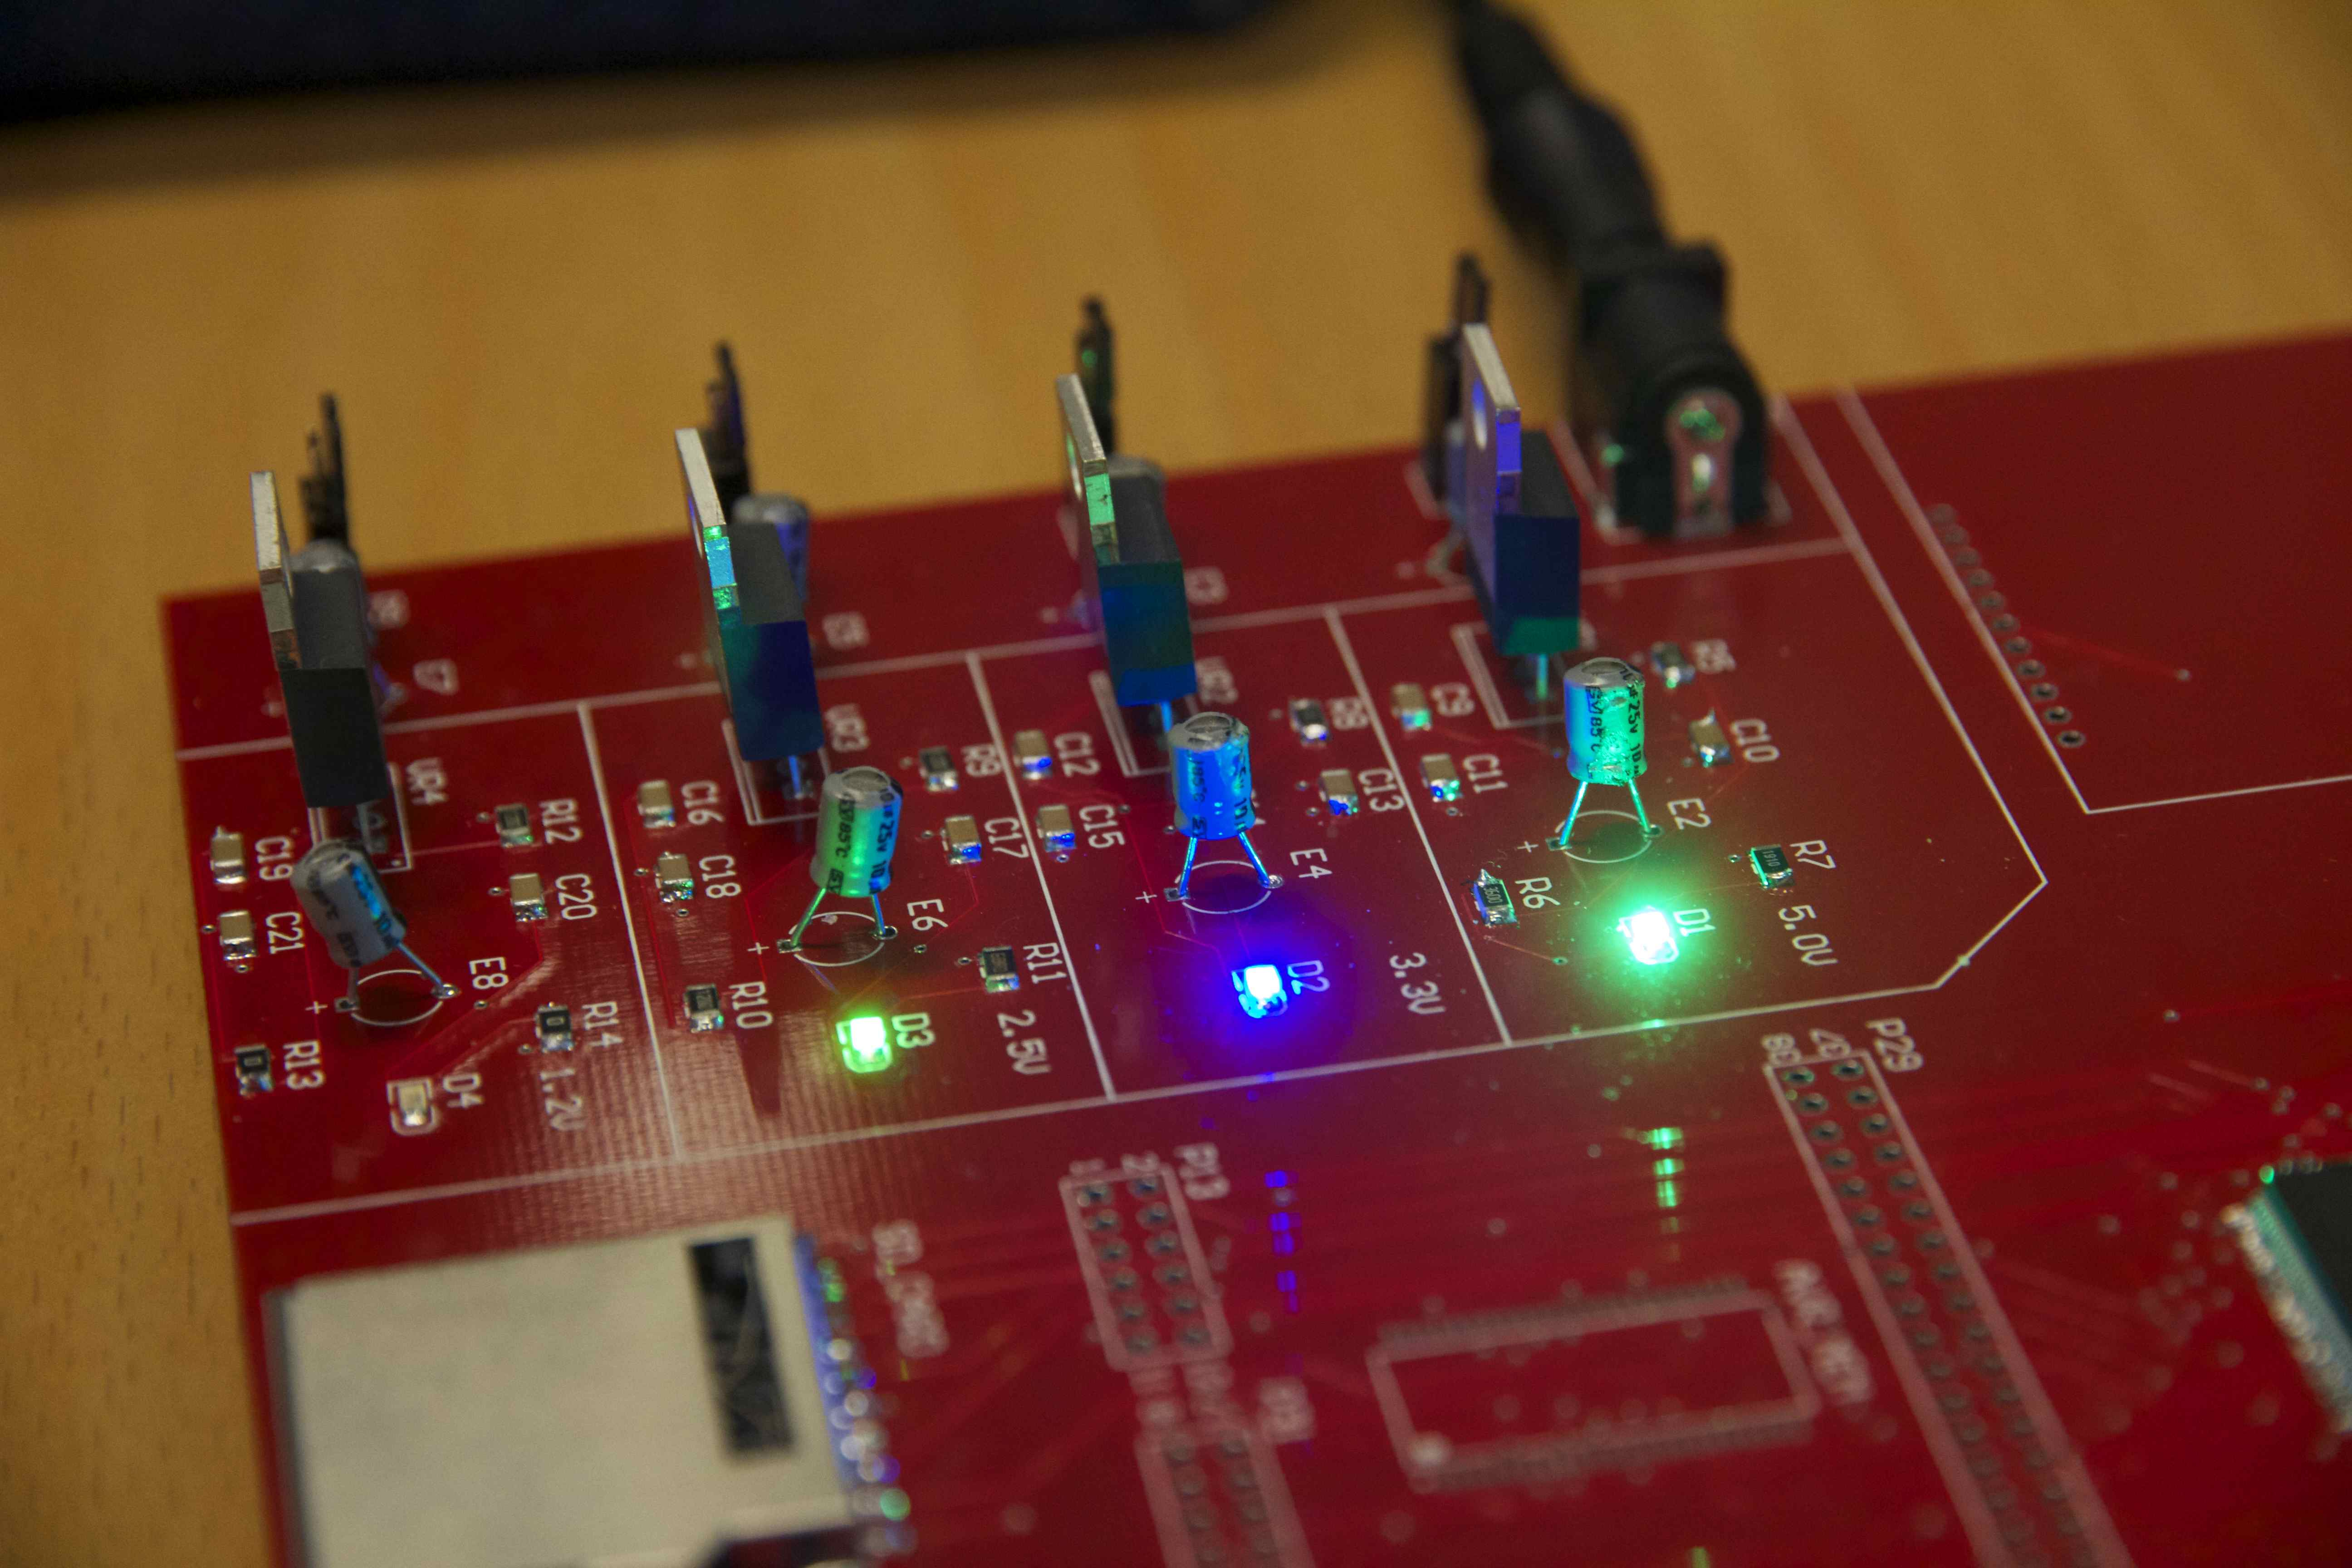
\includegraphics[width=0.8\textwidth]{fig/pcb/pcb_powersoldered.jpeg}
  \caption[The PCB Power Supply]{The PCB with the powersupply soldered.}
  \label{fig:pcb-powersoldered}
\end{figure}

After talking to Tufte and Jahre, we decided to reuse the power supply
from Festina Lente without any changes. Tufte said the power supply had evolved year by
year, and that it would therefore be a better solution to reuse it rather
than trying to create one from scratch. By doing so, we reduced the possibility 
of introducing new issues.

\section {Power plane}

\begin{figure}[h]
  \centering
  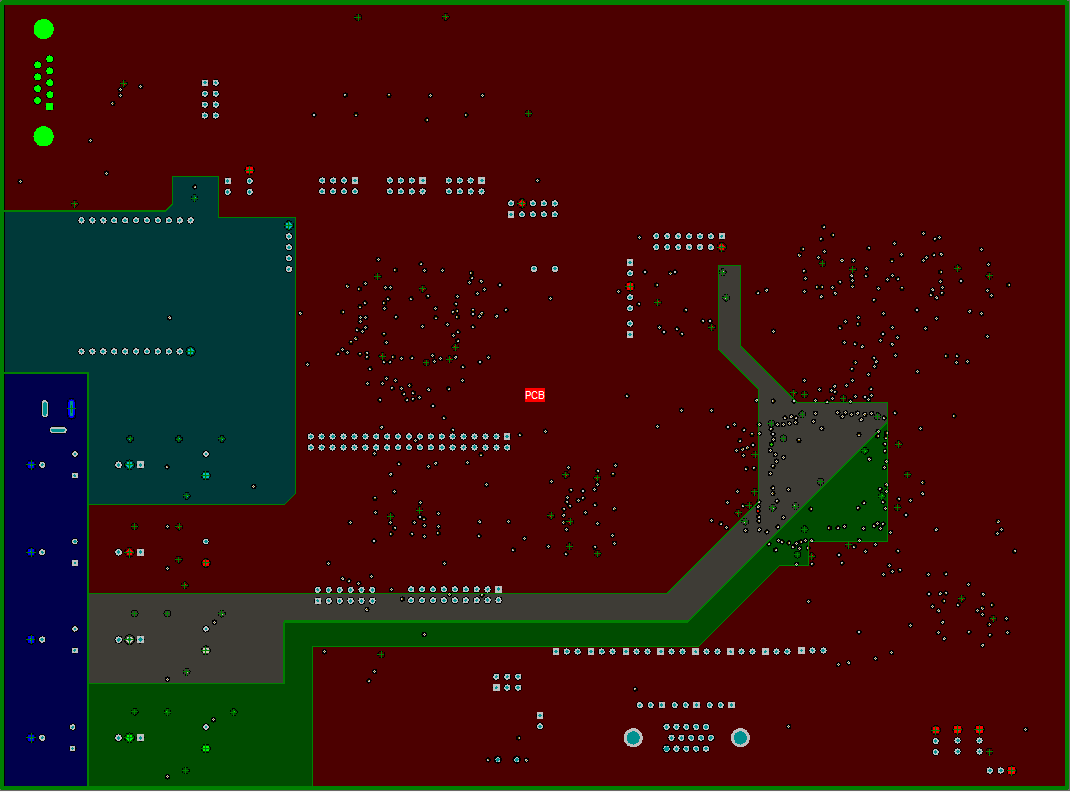
\includegraphics[width=0.8\textwidth]{fig/pcb/power_planes.PNG}
  \caption{The Power Planes}
  \label{fig:power_planes}
\end{figure}


Since our power supply was exactly the same as Festina Lente's we also ended up
with similar power planes, as seen on the figure above; 12V (dark blue), 5V (teal), 
3.3V (red), 2.5V (gray) and 1.2V (green). The 5V was only used for the external 
\ac{VGA} controller. 2.5V and 1.2V were split across the \ac{FPGA}.

The rest of the board got 3.3V. The entire power plane was put in internal layer
1, with a ground layer in internal layer 2.

\section {Footprints}
Some of the components we chose did not have footprints readily available, which
meant we either had to look for them on the internet, or create some ourselves.

This usually meant either staring at datasheets and carefully placing pins
relative to each other, or running the IPC-wizard.

\subsection {We made the following footprints ourselves}
\TODO{Make the links to references}
\begin {itemize}
\item SD-card \url{http://katalog.we-online.de/em/datasheet/693063010911.pdf}
  With the pin-designations selected by googling the pinouts for SD-cards in
  general, and comparing a few of those hits to make sure that the results
  agreed \url{http://pinouts.ru/Memory/sdcard_pinout.shtml} ended up being what
  we based the schematic-component based on. \CHECK{Mention that this was
    particularly hard to decipher from the datasheet, and that we did need to
    ask Gunnar for help at least once, just to read the datasheet?}
\item VGA-plug \url{http://www.te.com/commerce/DocumentDelivery/DDEController?Action=srchrtrv&DocNm=82068_AMPLIMITE_Right-Angle_Posted_Conn&DocType=Catalog+Section&DocLang=English&PartCntxt=}
\item Memory (TSOP54/TSOP44)
\TODO{Fill in a bit about the wizard used to generate this}
The TSOP54/TSOP44 footprints were created using the IPC Footprint Wizard, as
their datasheets fitted nicely with the Small Outline Package-setting in that
Wizard.

Data-memory (2M x 8bit) CY7C1069DV33 54TSOP:
\url{http://www.cypress.com/?docID=31945} Program-memory (64K x 16bit)
CY7C1021DV33 44TSOP: \url{http://www.cypress.com/?docID=31965} VGA memory (512 x
8bit) CY7C1049DV33 TSOP44 : \url{http://www.farnell.com/datasheets/1468461.pdf}
\end {itemize}

\subsection{Footprints from Festina Lente:}
As Festina Lente used some components that we also ended up using, we decided,
after talking to Gunnar\CHECK{Should we refer by first or last name?}, to use
their Footprints (as they were known good) for these components:
\url{http://org.ntnu.no/datamaskinerprosjekt2011/altium_libraries/dmprolibrary/}
\begin{itemize}
\item Button
\item Crystal
\item USB
\item Oscillator The oscillator had one issue last year, namely that the
  footprint was mirrored, noting this from Festina Lente's report, we read
  through the datasheet (REFERENCE)\TODO{Reference}, and remapped the
  pin-numbering on the foot-print before using this footprint.
\item PowerConnector
\item VGA-module
\end{itemize}
\CHECK{Molex? Still in the project, but wasn't used. Double-check this.}

In addition we used the following premade footprints:
\begin{itemize}
\item AVR-footprint | from AVR-freaks.
\item FPGA-footprint | Built-in from the Altium Designer Library.
\end{itemize}

\TODO{Mention the 1206-es that we chose to use based on the Festina
  Lente-report}

%Flytta til process
%\subsection {Routing}
\subsection {Routing}
\input{fig/pcb/routing}
We spent the entire final week before production working on the routing. In comparison, the energy group used only 2 days. There are quite a few possible reasons why we ended up using so much more time than them for this:

One of the reasons were simply that we were the first group to start routing. We thus got to fall into some gotcha-traps, with no one to warn us about them.

An example of such a trap was that we didn't set the correct Design Rules before auto-routing, until a few days into the week. This naturally didn't give us the routing that we wanted, and gave us a few headaches.

Related to this is the fact that we didn't experiment enough with different routing strategies. We wanted to reduce the number of vias, but went with the default routing in Altium. We then did quite an amount of manual routing to reduce the number of vias. Figure \ref{fig:removingvias-pcb} shows an example where we coupled together several pins to the same via going to the GND-layer. The amount of manual work could perhaps have been reduced by selecting the "Via Mixer" strategy instead.

\input{fig/pcb/pcb_removing_vias} \TODO{Write about this figure}

Another reason has to do with the difference between our designs. Where the other group had to route only 1 memory chip, we had 5. This naturally made the routing much more complex.

Initially we attempted auto routing. This took just around 12 minutes before constraints were set. And the better part of half an hour, after the constraints were set. This showed us quite a few issues that needed to be handled, and even more so when we finally got the constraints in.

\TODO{Fill in about the types of errors/warnings we got.}
\begin{itemize}
\item Constraints violations set wrong.
\item Power-plane net-labeled wrong.
\item Clearance constraints violated by Altium.
\item Short-circuiting vias.
\item Overlapping vias.
\item In general, the auto-routing started to produce violations.
\item more\ldots
\end{itemize}
\TODO{Silk-over-silk in USB/Lenna, errors we could ignore.}
\TODO{Scaling of board. (Should go elsewhere or not at all?)}

Initially we started with a board size chosen more or less at random, and picked something that seemed to fit the components comfortably with room to spare.

After laying out the components on the board, we noticed that the board had quite a bit of room left over. As this would be a waste of resources, we scaled the board down in size. We did this by moving the keep-out-borders inwards until the wasted space was removed, and then used the ``scale-to-fit-components''-tool in Altium, with the Keepout-border selected.

In the end we remapped some pins to increase physical proximity, and to untangle the amount of crossing wires. Although care was taken during this process, we accidentally happened to disconnect one pin in the schematic while reordering. We did notice this before production, and were able to correct the mistake by manually routing the connection. Finally, we did some manual routing to reduce the amount of unnecessary vias.


We spent the entire final week before production working on the routing. In comparison, the energy group used only 2 days. There are quite a few possible reasons why we ended up using so much more time than them for this:

One of the reasons were simply that we were the first group to start routing. We thus got to fall into some gotcha-traps, with no one to warn us about them.

An example of such a trap was that we didn't set the correct Design Rules before auto-routing, until a few days into the week. This naturally didn't give us the routing that we wanted, and gave us a few headaches.

Related to this is the fact that we didn't experiment enough with different routing strategies. We wanted to reduce the number of vias, but went with the default routing in Altium. We then did quite an amount of manual routing to reduce the number of vias. Figure \ref{fig:removingvias-pcb} shows an example where we coupled together several pins to the same via going to the GND-layer. The amount of manual work could perhaps have been reduced by selecting the "Via Mixer" strategy instead.

\begin{figure}[h]
  \centering
  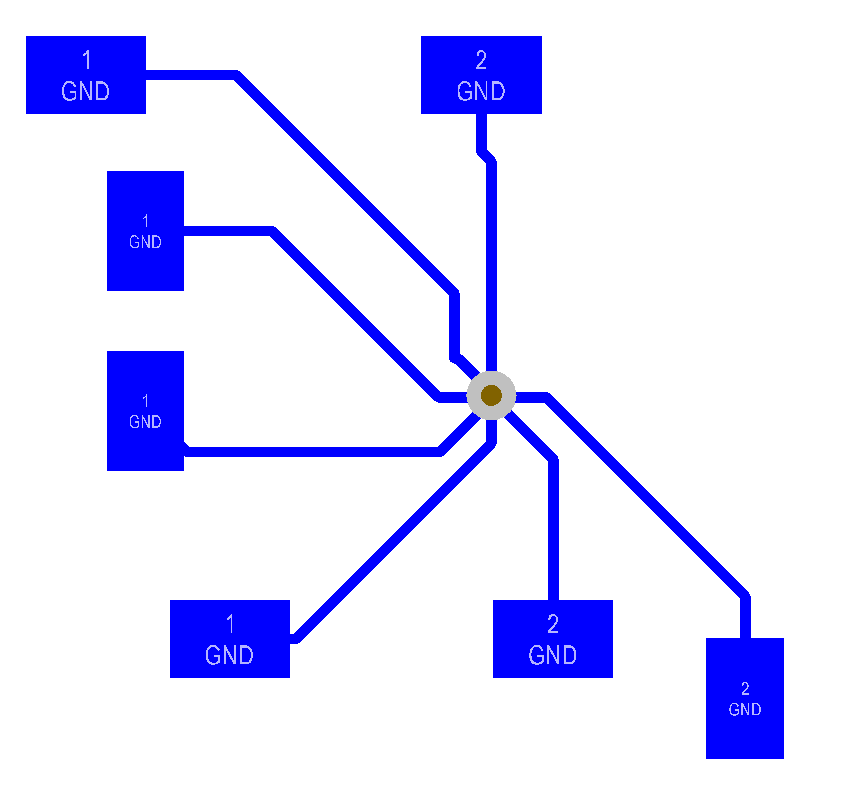
\includegraphics[width=0.8\textwidth]{fig/pcb/pcb_removing_vias.png}
  \caption{Removing vias}
  \label{fig:removingvias-pcb}
\end{figure}
 \TODO{Write about this figure}

Another reason has to do with the difference between our designs. Where the other group had to route only 1 memory chip, we had 5. This naturally made the routing much more complex.

Initially we attempted auto routing. This took just around 12 minutes before constraints were set. And the better part of half an hour, after the constraints were set. This showed us quite a few issues that needed to be handled, and even more so when we finally got the constraints in.

\TODO{Fill in about the types of errors/warnings we got.}
\begin{itemize}
\item Constraints violations set wrong.
\item Power-plane net-labeled wrong.
\item Clearance constraints violated by Altium.
\item Short-circuiting vias.
\item Overlapping vias.
\item In general, the auto-routing started to produce violations.
\item more\ldots
\end{itemize}
\TODO{Silk-over-silk in USB/Lenna, errors we could ignore.}
\TODO{Scaling of board. (Should go elsewhere or not at all?)}

Initially we started with a board size chosen more or less at random, and picked something that seemed to fit the components comfortably with room to spare.

After laying out the components on the board, we noticed that the board had quite a bit of room left over. As this would be a waste of resources, we scaled the board down in size. We did this by moving the keep-out-borders inwards until the wasted space was removed, and then used the ``scale-to-fit-components''-tool in Altium, with the Keepout-border selected.

In the end we remapped some pins to increase physical proximity, and to untangle the amount of crossing wires. Although care was taken during this process, we accidentally happened to disconnect one pin in the schematic while reordering. We did notice this before production, and were able to correct the mistake by manually routing the connection. Finally, we did some manual routing to reduce the amount of unnecessary vias.


\section {PCB testing}

\begin{figure}[h]
  \centering
  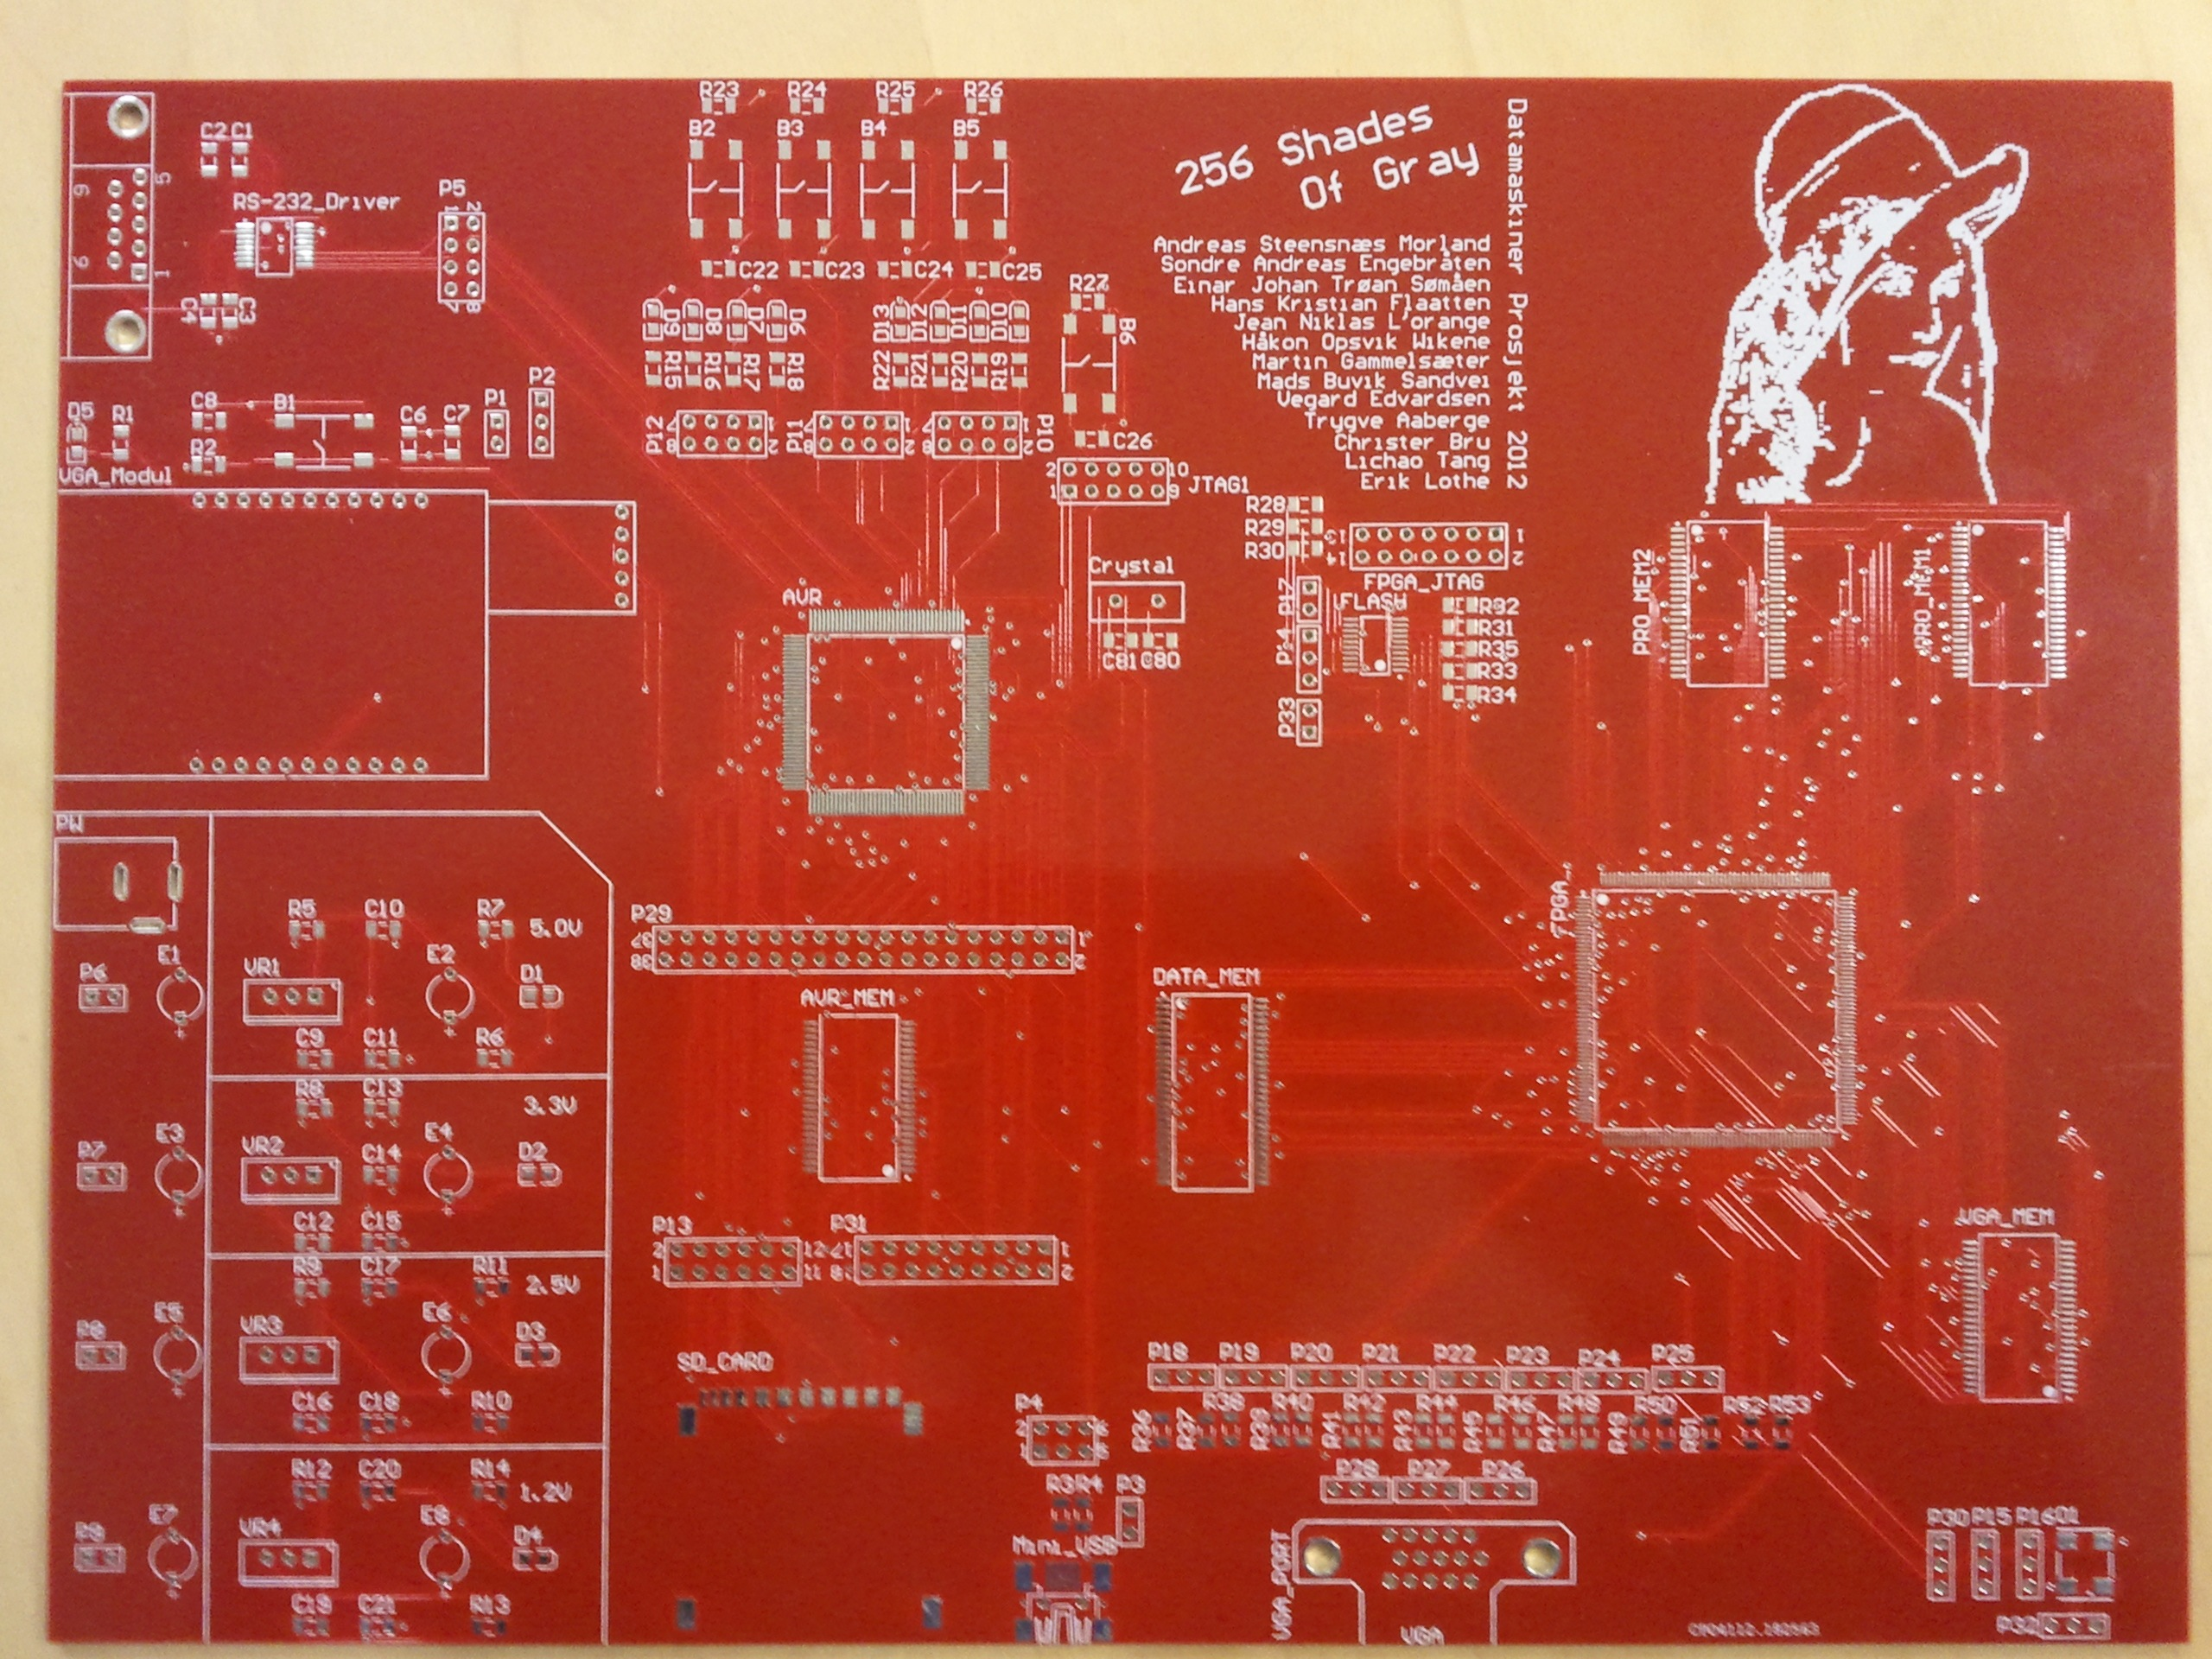
\includegraphics[width=0.8\textwidth]{fig/pcb/pcbwithoutcomp.jpg}
  \caption{The PCB Without Components}
  \label{fig:pcb-without-components}
\end{figure}


When the \ac{PCB} arrived from production, the soldering proved
to be a bit more difficult than originally anticipated.
First, we tested whether
there were any short circuits in the board itself. We used the multimeter to test that
there was no current passing from one layer to another. Then, we started to solder the power supply, one power plane at time, testing the board for short
circuit after each iteration. The table \ref{fig:pcb} shows the observed voltage from each plane.

\begin{table}[h]
  \centering
  \begin{tabularx}{\textwidth}{l l l l}\toprule
    \thx{Test} & \thx{Result} & \thx{Passed} 
    \\ 
	 \midrule
    Power supply 12.0V               &Measured 12.045  & OK  \\	
\midrule
    Power supply 5.0V               &Measured 4.995  & OK  \\
    \midrule
    Power supply 3.3V                   & Measured 3.286 & OK  \\
    \midrule
    Power supply 2.5V                 & Measured 2.510 & OK \\
    \midrule
    Power supply 1.2V            & Measured 1.240 & OK  \\
    
    \bottomrule
  \end{tabularx}
  \caption{Results of power supply}
  \label{fig:pcb}
\end{table}


\begin{figure}[h]
  \centering
  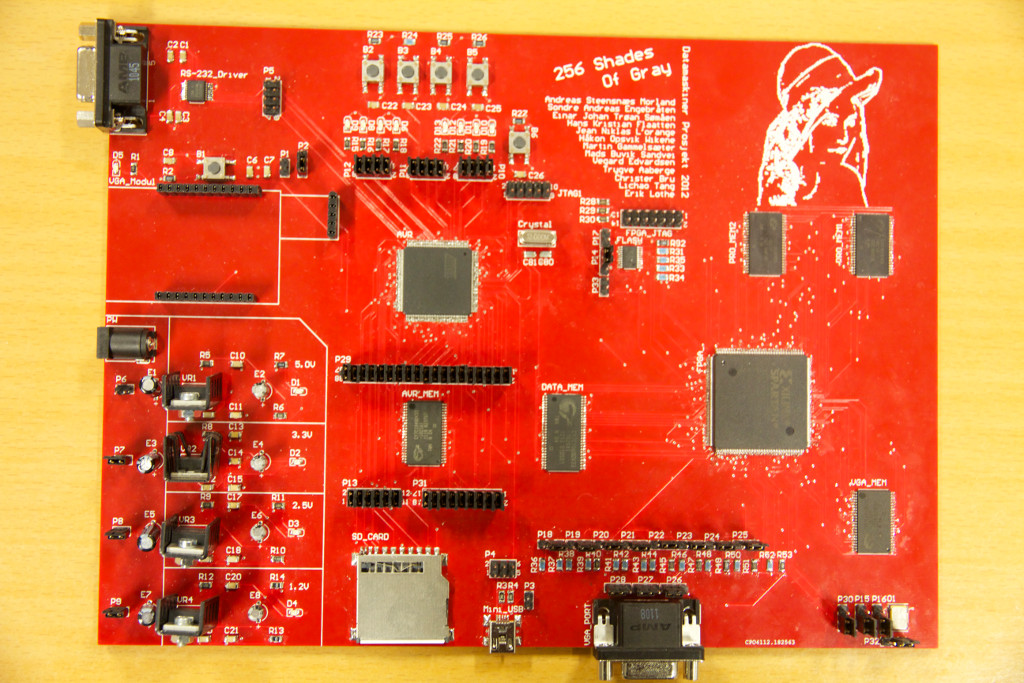
\includegraphics[width=0.8\textwidth]{fig/pcb/pcbwithcompnew.jpeg}
  \caption[The PCB]{The PCB With All The Components.}
  \label{fig:pcb-with-components}
\end{figure}


\section {Process}
This section describes the work and design challenges faced related to the PCB.
\subsection{Memory}
As discussed earlier, as one of our earliest design choices we chose 3 separate memories to allow overlap of
memory accesses. Since the requirements for the data/instruction memories differed in both size and word-width 
we wound up with not only separate, but also different chips for this purpose. The same choice meant we also
needed a separate memory for our \ac{VGA} controller, as that needed to read it's buffer as fast as possible
without interfering with the speed of the rest of the system. This called for a memory that was big enough to
hold atleast a full screen-frame, at 8-bit per pixel (since each pixel is an 8-bit greyscale pixel).

To reduce the possibility of having too slow data-access from the AVR, an extra memory was added to work as
a buffer for the AVR as well. This design choice was made {\em after} ordering, which meant that we had to choose from
the chips we had already ordered to fit this purpose. Since this was intended to carry data intended for the rest
of the system, and as the rest of the system is working with data in 8-bit bytes, we ended up using one of the
extra chips ordered as \ac{VGA} memory for this purpose.

\subsection {Schematics}
The workflow of creating the schematic consisted of reading data sheets,
and looking at the reports from earlier computer design projects, and then
applying the knowledge we found from those to properly place the necessary
components in our schematic.

We decided to design the entire \ac{PCB} in one schematic, as the Festina Lente
report mentioned that Festina Lente-report does mention that 
``The decision to make the central components appear in multiple schematic
sheets made Altium issue a lot of warnings and errors during the design rule 
check''\cite[p.~49]{berg2011festinalente}. Something we avoided from day one, 
as we never attempted to use multiple schematics-documents.

A downside of this approach was the fact that this partially serialized
our work on the schematic, since we could not make concurrent changes to our
single document. When not working on the schematic, the other people in the
\ac{PCB} group did whatever could be done without touching the
schematic. (Making footprints, verifying design, looking up parts and data
sheets) Since the schematic was the biggest amount of work, this produced
something of a bottleneck for the PCB work.

However, having overall control of the entire thing in one document
did help to smooth out some issues we met while working. For instance,
we were having quite a few issues with net labels. This was quite easy to
solve when everything was in one document with no ports, as getting
complete overview was doable, without having to cross-reference schematics.
We also avoided the need to use any buses, although we did end up adding
some for the sake of readability.

The overall layout of the Schematic \ref{app:schematics} is logically grouped ``geographically'', to
allow for easy reading of the schematic.

\subsubsection {Buses/Wirelabels}
We initially worked from the assumption that all pins should be connected to a
bus, and then that bus should be connected to the pins in the other end. This
gave us some issues with duplicate naming. After digging through quite a bit of
Altium documentation, we became assured that simply wire-labeling the pins
would create the necessary connections. This is because any pin/wire with the
same name as any other pin/wire will be connected by definition in Altium.

This arguably made for a less readable schematic, as the bus-connected solution
was quite a lot easier to follow when tracing. However, as our schematic still
is logically grouped, it is not very hard to find the correct connections even
without the buses drawn in. We are quite sure that given a logical overview of
which components are directly connected to each other, finding the various pins
that perform this connection should be trivial even without the buses/wires
drawn in.


\subsection {Routing}
\subsection {Routing}
\input{fig/pcb/routing}
We spent the entire final week before production working on the routing. In comparison, the energy group used only 2 days. There are quite a few possible reasons why we ended up using so much more time than them for this:

One of the reasons were simply that we were the first group to start routing. We thus got to fall into some gotcha-traps, with no one to warn us about them.

An example of such a trap was that we didn't set the correct Design Rules before auto-routing, until a few days into the week. This naturally didn't give us the routing that we wanted, and gave us a few headaches.

Related to this is the fact that we didn't experiment enough with different routing strategies. We wanted to reduce the number of vias, but went with the default routing in Altium. We then did quite an amount of manual routing to reduce the number of vias. Figure \ref{fig:removingvias-pcb} shows an example where we coupled together several pins to the same via going to the GND-layer. The amount of manual work could perhaps have been reduced by selecting the "Via Mixer" strategy instead.

\input{fig/pcb/pcb_removing_vias} \TODO{Write about this figure}

Another reason has to do with the difference between our designs. Where the other group had to route only 1 memory chip, we had 5. This naturally made the routing much more complex.

Initially we attempted auto routing. This took just around 12 minutes before constraints were set. And the better part of half an hour, after the constraints were set. This showed us quite a few issues that needed to be handled, and even more so when we finally got the constraints in.

\TODO{Fill in about the types of errors/warnings we got.}
\begin{itemize}
\item Constraints violations set wrong.
\item Power-plane net-labeled wrong.
\item Clearance constraints violated by Altium.
\item Short-circuiting vias.
\item Overlapping vias.
\item In general, the auto-routing started to produce violations.
\item more\ldots
\end{itemize}
\TODO{Silk-over-silk in USB/Lenna, errors we could ignore.}
\TODO{Scaling of board. (Should go elsewhere or not at all?)}

Initially we started with a board size chosen more or less at random, and picked something that seemed to fit the components comfortably with room to spare.

After laying out the components on the board, we noticed that the board had quite a bit of room left over. As this would be a waste of resources, we scaled the board down in size. We did this by moving the keep-out-borders inwards until the wasted space was removed, and then used the ``scale-to-fit-components''-tool in Altium, with the Keepout-border selected.

In the end we remapped some pins to increase physical proximity, and to untangle the amount of crossing wires. Although care was taken during this process, we accidentally happened to disconnect one pin in the schematic while reordering. We did notice this before production, and were able to correct the mistake by manually routing the connection. Finally, we did some manual routing to reduce the amount of unnecessary vias.


We spent the entire final week before production working on the routing. In comparison, the energy group used only 2 days. There are quite a few possible reasons why we ended up using so much more time than them for this:

One of the reasons were simply that we were the first group to start routing. We thus got to fall into some gotcha-traps, with no one to warn us about them.

An example of such a trap was that we didn't set the correct Design Rules before auto-routing, until a few days into the week. This naturally didn't give us the routing that we wanted, and gave us a few headaches.

Related to this is the fact that we didn't experiment enough with different routing strategies. We wanted to reduce the number of vias, but went with the default routing in Altium. We then did quite an amount of manual routing to reduce the number of vias. The amount of manual work could perhaps have been reduced by selecting the "Via Mixer" strategy instead.

\TODO{Insert "via-hub" figure here}

Another reason has to do with the difference between our designs. Where the other group had to route only 1 memory chip, we had 5. This naturally made the routing much more complex.

Initially we attempted autorouting. This took just around 12 minutes before constraints were set. And the better part of half an hour, after the constraints were set. This showed us quite a few issues that needed to be handled, and even more so when we finally got the constraints in.

\TODO{Fill in about the types of errors/warnings we got.}
\begin{itemize}
\item Constraints violations set wrong.
\item Power-plane net-labeled wrong.
\item Clearance constraints violated by Altium.
\item Short-circuiting vias.
\item Overlapping vias.
\item In general, the auto-routing started to produce violations.
\item more\ldots
\end{itemize}
\TODO{Silk-over-silk in USB/Lenna, errors we could ignore.}
\TODO{Scaling of board. (Should go elsewhere or not at all?)}

Initially we started with a board size chosen more or less at random, and picked something that seemed to fit the components comfortably with room to spare.

After laying out the components on the board, we noticed that the board had quite a bit of room left over. As this would be a waste of resources, we scaled the board down in size. We did this by moving the keep-out-borders inwards until the wasted space was removed, and then used the ``scale-to-fit-components''-tool in Altium, with the Keepout-border selected.

In the end we remapped some pins to increase physical proximity, and to untangle the amount of crossing wires. Although care was taken during this process, we accidentally happened to disconnect one pin in the schematic while reordering. We did notice this before production, and were able to correct the mistake by manually routing the connection. Finally, we did some manual routing to reduce the amount of unneccessary vias.

\subsection{Soldering}
After that we started soldering the AVR. Getting the AVR in place was particularly difficult,
but after asking Tufte, we lent a glue stick to put some glue on. The increased friction helped keeping the AVR in place during soldering.

After about a days work we managed to completely destroy a pin on the AVR,
therefore we had to start from scratch on a new board. On this new board we
started with the AVR and \ac{FPGA}, as they were the hardest components to
solder. After each side on the AVR and \ac{FPGA}, we tested for short
circuits. As none were found, we moved on to the power supply, as well as
\acp{JTAG}, FLASH and \acp{LED}. In order to check the \ac{PCB} was working, the
AVR and \ac{FPGA} groups tested the \ac{PCB} board without the capacitors, after
both groups tested that they could connect to the AVR and \ac{FPGA}
respectively, we began to solder the rest part of the \ac{PCB}.


\section {Problems and Workarounds}
\subsection{Routing}
Routing was the first problem we confronted during the designing the \ac{PCB}
board, we had to manually route the design, because we got some warnings due to
the clearance of the board. We used the auto-routing function provided by
Altium, yet as it did not provide satisfying results, we tried to change some
parameters to make them better, without success. Finally, we realized that we
had to route a few wires manually. This was mostly motivated by our desire to
not have vias as close to the pins as Altium placed them. Also, as to cut down
the budget, we removed some unnecessary vias by wiring multiple grounds and
powers together, where the design allowed us to. In this way, we got quite a few
less vias.

We spent the entire final week before production working on the routing. In comparison, the energy group used only 2 days. There are quite a few possible reasons why we ended up using so much more time than them for this:

One of the reasons were simply that we were the first group to start routing. We thus had no one to warn us about mistakes. An example of such a mistake was that we did not set the correct Design Rules before auto-routing, until a few days into the week. This naturally did not give us the routing that we wanted, and gave us a few headaches.

Related to this is the fact that we did not experiment enough with different routing strategies.

Another reason relates to the difference between our designs. Where the other group had to route only 1 memory chip, we had 5. This naturally made the routing much more complex.
\subsection{Soldering}
Soldering was the biggest problem that we faced, none of the \ac{PCB} group
member had any experiences with it beforehand. We managed to destroy our first
board, as we used too much tin on one of the AVR pins, and ruined them by using
the tin removal unit wrongly.

The next try, however, proved to be successful, but there still remained some
minor problems. Problems we found were lack of tin on the oscillator, as well as
a few of the \ac{FPGA} pins. They were, as opposed to our problem with the first
board, easily fixed, once discovered.





\chapter{System Testing}\label{ch:sys-test}

\begin{flushright}{\slshape
    In which a set of tests are designed,\\
    carefully and ingeniously to confirm or reject\\
    the functional requirements we have designed
}
\end{flushright}

Any system with functional requirements needs to verify whether the functional
requirements are satisfied or not. This is done through system tests, which are
essential to get a confirmation or a rejection on whether we satisfy the
requirements. Usually will test the functionality of a system as a whole, but
the nature of our requirements\TODO{Are they really like this?} means that some
of the tests will only test specific parts of the system. 

This chapter will start by presenting the design of the system tests. It will
then go into how we will test the different tests. We summarize by presenting
our results with additional comments.


\chapter{Results}


\chapter{Discussion}\label{ch:disc}

\begin{flushright}{\slshape
    In which we explain the path we took at junctions\\
    what waypoints we looked at,\\
    and where we could be if we changed course
}
\end{flushright}

\chapter{Conclusion}\label{ch:conc}

\begin{flushright}{\slshape
    In which a conclusion is reached\\
    where ideas and theories\\
    peeks on reality
}
\end{flushright}

This part seems relatively straightforward, and will be written in the
not-to-distant future.

\section{Conclusion}

\begin{itemize}
\item If we removed the special ``Get all 4 neighbour values at
  once''-instructions and other special parts of the system, would we be able to
  get more cores?
\item If we strip the SIMD nodes almost to the bone, barely being turing
  complete, how many nodes would we get?
\end{itemize}

\section{Future Work}


\appendix

 % NB: SHOULD NOT BE A CHAPTER. SHOULD BE APPENDIX. TODO: hyPiRion
\chapter{Ordered parts}
Prices and pieces

\begin{table}[h]
  \centering
  \begin{tabularx}{\textwidth}{l c r r r}\toprule
    \thx{Name} & \thx{Product ID} & \thx{Count} & \thx{Price} & \thx{Total}
    \\ \midrule
    SD card reader               & 2081360 & 2 &  38,78 kr &  77,56 kr \\
    \midrule
    Serial port                  & 1653975 & 2 &   8,63 kr &  17,26 kr \\
    \midrule
    Serial driver                & 1287435 & 2 &  24,25 kr &  48,50 kr \\
    \midrule
    USB port (Mini B)            & 1243250 & 2 &  17,89 kr &  35,78 kr \\
    \midrule
    VGA controller               & ??????? & 1 &   0,00 kr &   0,00 kr \\
    \midrule
    VGA port                     & 1056018 & 2 &  91,61 kr & 183,22 kr \\
    \midrule
    Data memory\\ (2M x 8bit)      & 2115432 & 2 & 326,02 kr & 652,04 kr \\
    \midrule
    Program memory\\ (64K x 16bit) & 2115418 & 3 &  19,85 kr &  59,55 kr \\
    \midrule
    VGA memory\\ (512 x 8bit)      & 1688739 & 2 &  57,43 kr & 114,86 kr \\
    \bottomrule
  \end{tabularx}
  \caption{Components}
  \label{fig:components}
\end{table}




\bibliographystyle{plain}
\bibliography{bibliography}

\end{document}
